\documentclass{article}

\PassOptionsToPackage{numbers, sort&compress}{natbib}
\usepackage[final,sglblindworkshop]{neurips_2025}
\workshoptitle{2nd Workshop on Principles of Generative Modeling (PriGM)}
% The 2026 CFP links the unmodified 2025 style. Only the venue notice is updated.
\makeatletter
\renewcommand{\@noticestring}{40th Conference on Neural Information Processing Systems (NeurIPS 2026) Workshop: 2nd Workshop on Principles of Generative Modeling (PriGM).}
\makeatother

\usepackage[utf8]{inputenc}
\usepackage[T1]{fontenc}
\usepackage{hyperref}
\usepackage{url}
\usepackage{booktabs}
\usepackage{amsfonts}
\usepackage{amsmath}
\usepackage{microtype}
\usepackage{graphicx}
\usepackage{orcidlink}
\hypersetup{colorlinks=false,pdfborder={0 0 1},linkbordercolor={1 0 0},citebordercolor={0 1 0},urlbordercolor={0 1 1},pdfauthor={Kevin Lee},pdftitle={Residual Penalties Versus Algebraic Completion In Conditional Diffusion},pdfsubject={},pdfkeywords={}}

\title{Residual Penalties Versus Algebraic Completion In Conditional Diffusion}
\author{%
 Kevin Lee{\hypersetup{hidelinks}\orcidlink{0009-0004-0388-9260}} \\
 [4pt]
 University of California at Los Angeles \\
 NASA Jet Propulsion Laboratory \\
 [2pt]
 \texttt{kevinlee69720@g.ucla.edu}
}

\begin{document}
\maketitle

\begin{abstract}
Missing solar wind measurements leave uncertainty in both the mean magnetic field and its fluctuations. These quantities obey an exact variance identity. Conditional diffusion experiments examine how enforcing this identity changes the predicted distribution. A residual penalty improves the score at the final training update, but most of its mean advantage disappears when validation chooses the model. Generating fewer variables and completing the rest algebraically gives the lowest mean energy score among the methods tested, with changes to both representation and loss. Its intervals still cover too few measurements. Clipping existing samples can worsen the score through a loss of ensemble spread. In an example with a known conditional distribution, a short sampling approximation using an exact denoiser gives small residuals but inaccurate probabilities. These comparisons connect constraint enforcement to its effects during training and sampling, showing how algebraic consistency can coexist with errors in predictive uncertainty.
\end{abstract}

\section{Introduction}

Missing solar wind measurements complicate estimates of magnetic turbulence \citep{wrench2022statistics}. Large vectors pointing in different directions can have a small mean, so reconstructing the mean field leaves its fluctuations uncertain. Here, conditional diffusion infers the joint distribution of six magnetic statistics throughout a missing hour, using measurements before and after it. They describe the mean field, magnitude and variances in successive bins of five minutes.\footnote{Available at: \url{https://github.com/magnaprog/diffusion-consistency}}

An exact variance identity determines one statistic from the other five. It holds for arbitrary vectors, independently of plasma dynamics, and allows many conditional distributions. Uncertainty complicates its use during training: the exact conditional mean can have a nonzero residual even though every realization satisfies the identity.

The experiments use conditional diffusion \citep{tashiro2021csdi} with the residual objective and sampling approximation of Physics-Informed Diffusion Models \citep{bastek2025pidm}. Earlier work studies residual minimization and distribution matching \citep{baldan2025physics}, or constructs outputs satisfying algebraic constraints \citep{beucler2021constraints}. Here, the comparisons distinguish a penalty during training, generation in fewer coordinates, and transformation of existing samples. Several training stages and an example with a known conditional distribution reveal how these operations affect consistency and predictive accuracy.



\section{Magnetic statistics and data}

Let $B_j$ denote five consecutive OMNI vector averages, each over one minute, from the same spacecraft in geocentric solar ecliptic coordinates. Define
\begin{equation}
 \mu=\frac15\sum_j B_j,\quad m=\frac15\sum_j\|B_j\|,\quad
 v_s=\frac15\sum_j(\|B_j\|-m)^2,\quad
 v_v=\frac15\sum_j\|B_j-\mu\|^2.
\end{equation}
The variances describe fluctuations in magnitude and in the vector, respectively, among the minute averages. The six variables are $z=(\mu_x,\mu_y,\mu_z,m,v_s,v_v)$. Expanding both population variances gives
\begin{equation}
 R_{\mathrm{obs}}(z)=m^2+v_s-\|\mu\|^2-v_v=0.
 \label{eq:identity}
\end{equation}
Omitting the variances gives $R_{\mathrm{inst}}=m^2-\|\mu\|^2$. For realizable statistics, it measures directional cancellation, weighted by field amplitude. It vanishes when all nonzero vectors share a direction, even if their magnitudes differ. Reducing amplitudes while retaining their directions can also lower this residual.

Write $r=\|\mu\|$. Five vectors in three dimensions, including possible zero vectors, can realize these statistics exactly when
\begin{equation}
 m\ge r,\qquad 0\le v_s\le\frac32m^2+\frac52r^2,\qquad
 v_v=m^2+v_s-r^2.
 \label{eq:support}
\end{equation}
Appendix~\ref{app:support} proves sufficiency. The equality and inequalities play different roles. Deriving $v_v$ enforces the equality while preserving the other five variables and their primary score. Clipping also brings $m$ and $v_s$ into the ranges in Equation~\ref{eq:support}, which can change that score.

The same identity behaves differently when applied to a conditional mean. For conditioning information $Y$,
\begin{equation}
 R_{\mathrm{obs}}(\mathbb{E}[z\mid Y])
 =\operatorname{tr}\operatorname{Cov}(\mu\mid Y)-\operatorname{Var}(m\mid Y).
 \label{eq:conditional}
\end{equation}
Either sign is possible, even when every possible sample satisfies the identity. Thus, a nonzero residual at the denoiser's mean prediction can arise from conditional uncertainty. Evaluating residuals at individual samples instead checks the algebraic relation in each possible realization \citep{bastek2025pidm}.

\paragraph{Data construction.} OMNI combines solar wind measurements from several spacecraft \citep{king2005solar}. The inputs here come from its modified high resolution product \citep{nasamodifiedomni}, whose timestamps estimate arrival at the bow shock nose \citep{papitashvili2020omni}. Propagation and averaging precede masking, so the reconstruction concerns this arrival-time record. Magnitudes are Euclidean norms of the vector components. Each window spans four hours in 48 bins of five minutes. Masking the central twelve bins leaves 90 minutes of conditioning data on each side. Complete windows use one spacecraft within one month, retaining 12.77\% of possible training starts.

In each year from 2005 through 2024, training uses 15 January through 30 June, test uses August and September, and validation uses 1 November through 17 December. The intervening dates separate the sets. Normalization uses distinct training bins. Evaluation uses windows without overlap and limits their number per month, giving 319 validation and 480 test windows (Appendix~\ref{app:quality}).

\section{Models and evaluation}

\paragraph{Training.} D uses diffusion to generate all six variables \citep{ho2020ddpm}. I-S adds a penalty on $R_{\mathrm{inst}}$; O-S adds one on the variance identity $R_{\mathrm{obs}}$. G5 generates five variables and derives $v_v$ after sampling. All four models receive all six variables in the available intervals. Training and sampling add noise only within the missing hour and preserve the available measurements.

For standardized state $u$ in the missing hour, the training objective adapts \citet{bastek2025pidm} by combining mean squared error, weighted by Min-SNR-5 \citep{hang2023minsnr}, with a residual term:
\begin{equation}
 \mathcal L_t=w_t\,\operatorname{MSE}(\hat u_0,u_0)
 +\frac{c_R}{2\Sigma_t}\,\frac1{12}\sum_{k=1}^{12}
 \left(\frac{R(z^*_{0,k})}{B_{\mathrm{ref}}^2}\right)^2.
\end{equation}
Here $\hat u_0$ estimates the original signal. Two denoiser evaluations give $z^*_{0,k}$ in physical units, except at $t=1$, where the first estimate is reused. The data weight is $w_t=\min(\operatorname{SNR}_t,5)$; $\Sigma_t$ is the diffusion posterior variance, with $\Sigma_1:=\Sigma_2$. The scale $B_{\mathrm{ref}}^2$ averages $m^2+v_s$ over distinct training bins. A cosine schedule uses 100 steps \citep{nichol2021improved}. D and G5 use $c_R=0$; I-S and O-S use $c_R=0.0005$.

Three training seeds and five checkpoints per seed span the same update counts for each method (Appendix~\ref{app:protocol}). The penalty adds denoiser evaluations and computational cost. The test period had been examined during earlier development; the comparison retains the original settings and penalty coefficient without further tuning on that period.

\paragraph{Scores and uncertainty.} The energy score measures joint predictive accuracy through Euclidean distances; lower scores are better \citep{gneiting2007strictly}. The primary score uses $(\mu_x,\mu_y,\mu_z,m,v_s)$ at twelve hidden positions after TRAIN standardization. For $K$ independent samples, its unbiased estimate subtracts half their mean distance over $K(K-1)$ ordered pairs of distinct members from their mean distance to the withheld values. These terms assess proximity to measurements and ensemble spread. Monthly means receive equal weight. Continuous ranked probability scores, interval coverage and width assess individual coordinates (Appendix~\ref{app:protocol}).
Diffusion results average three training seeds, with coverage calculated separately for each ensemble. Intervals for score differences resample years or consecutive groups of two years, with replacement and common resamples for both methods. They describe temporal variation for the existing fits and samples. Subgroups defined by withheld outcomes are retrospective.

\paragraph{Model selection and baselines.} Validation compares ensembles of 39 samples from 25 denoising diffusion implicit model (DDIM) evaluations with $\eta=0$ \citep{song2021ddim}. It minimizes the energy score with equal month weights, choosing checkpoints separately before and after clipping; ties favor the earlier state. Test ensembles use 39 samples and 50 evaluations.

Linear interpolation joins the adjacent measurements; persistence repeats the preceding bin. Gaussian interpolation adds a residual fit on TRAIN with covariance shrinkage $\rho=0$. Gaussian regression uses the full available context and a common residual covariance, then derives $v_v$; validation chooses its ridge and covariance shrinkage parameters (Appendix~\ref{app:extension}).

\begin{table}[!b]
\centering
\caption{Results for 480 test windows with equal month weights. Energy scores use the 60 standardized primary coordinates. Diffusion results average three fits; each other baseline uses one ensemble realization. Validation selects checkpoints separately for raw and clipped diffusion predictions. Coverage is averaged over five primary variables at twelve hidden positions. $|R|$ is mean absolute $R_{\mathrm{obs}}$ in nT$^2$. The last column gives the percentage of bins that fail a moment inequality beyond rounding, excluding the equality test. Interpolation and persistence have intervals of zero width.}
\label{tab:main}
\begin{tabular}{lrrrrrr}
\toprule
 & \multicolumn{2}{c}{Energy score} & \multicolumn{2}{c}{90\% coverage (\%)} & \multicolumn{2}{c}{Raw samples} \\
Procedure & Raw & Clipped & Raw & Clipped & $|R|$ & \parbox[c]{19mm}{\centering Bins failing inequalities (\%)} \\
\midrule
D & 1.888 & 1.869 & 72.8 & 71.0 & 2.956 & 50.4 \\
I-S & 1.882 & 1.876 & 69.4 & 69.6 & 3.732 & 37.8 \\
O-S & 1.885 & 1.866 & 70.0 & 71.1 & 2.680 & 55.7 \\
G5 & 1.785 & 1.784 & 75.7 & 75.8 & 0.000 & 48.8 \\
Interpolation & 2.393 & 2.393 & 0.0 & 0.0 & 3.459 & 0.0 \\
Persistence & 3.067 & 3.067 & 0.1 & 0.1 & 0.000 & 0.0 \\
Gaussian interpolation & 2.125 & 2.229 & 94.3 & 93.6 & 15.491 & 77.7 \\
Gaussian regression & 1.935 & 2.035 & 94.0 & 93.5 & 0.000 & 74.6 \\
\bottomrule
\end{tabular}
\end{table}

\section{Results and interpretation}

Validation leaves little mean score difference between O-S and D (Table~\ref{tab:main}, Figure~\ref{fig:overview}a). O-S minus D is $-0.0028$, with a 95\% interval of $[-0.0346,0.0242]$ from resampling years. Relative intervals from both resampling schemes lie within the original $\pm2\%$ comparison range for these three fits. At the final update, however, O-S with the original coefficient has a lower raw score than D for all three seeds. Validation favors earlier D models, reducing this mean advantage.

G5 has the lowest mean primary score: O-S minus G5 is 0.1002, with interval $[0.0712,0.1391]$ from resampling years. Both the O-S/D and O-S/G5 comparisons reverse sign across seeds. Most of G5's mean improvement over D comes from the spread term in the score, with different contributions at each seed (Figure~\ref{fig:calibration}). Its intervals still cover too few measurements, especially for variance in field magnitude (Figure~\ref{fig:overview}b), and nearly half of its raw bins fail the moment inequalities. The lower score concerns a different representation and training loss. Algebraic completion alone preserves the other five quantities, so deriving $v_v$ from the same samples would leave their primary score intact.



\begin{samepage}
The effect of clipping depends on how far it moves the samples and how it changes their spread (Table~\ref{tab:operators}). G5's samples move, yet their mean energy score changes little. For Gaussian interpolation, clipping brings samples closer to the withheld measurements but reduces the spread term by more, increasing the score. For D, the change in Table~\ref{tab:main} also includes a different choice of checkpoint (Figure~\ref{fig:operator}).
\par
\end{samepage}

An exact denoiser isolates error in the sampling approximation (Figure~\ref{fig:hmm}). In a stationary hidden Markov model, it integrates over the unknown switching probability. New hidden paths and forward noise for each available context give a distribution of estimates. Across 36 cases at $t=100$, two evaluations give mean absolute $R_{\mathrm{obs}}=4.17\times10^{-5}$ in HMM units, yet energy score 6.958 versus 4.164 for independent exact conditional samples. Separately, DDIM sampling on 288 windows gives a poor score with two evaluations and scores close to that of the exact conditional ensemble with 25, 50, or 100 (Table~\ref{tab:oracle}). The residual estimate used in training and the full sampler have different accuracy here. All scores have finite sampling error.

\begin{figure}[t]
 \centering
 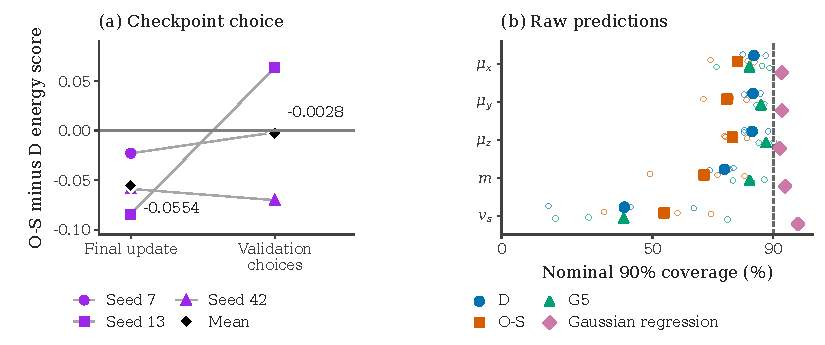
\includegraphics[width=\linewidth]{figures/overview/fig_overview.pdf}
 \caption{Model choice and predictive uncertainty. (a) O-S minus D energy score at the final update and at the checkpoints chosen independently by raw validation score. Symbols distinguish the three training seeds; diamonds show their mean. Negative values favor O-S. Validation with 25 or 50 evaluations chooses the same six checkpoints. (b) Raw nominal 90\% interval coverage for each magnetic quantity. Large filled markers average three diffusion fits; small open circles show individual fits. Gaussian regression uses one ensemble per window. The dashed line marks 90\%. Scores and coverage give equal weight to months; coverage also averages the twelve hidden positions.}
 \label{fig:overview}
\end{figure}

\section{Conclusion}

Algebraic constraints describe each possible realization; conditional prediction assigns probabilities to those realizations. The comparisons connect the effect of enforcing an identity to changes in training, representation and sampling. G5's lower score accompanies undercoverage, while clipping and the exact denoiser example show why a small residual can accompany an inaccurate distribution. Evaluating these operations involves both the moment relations and the uncertainty they produce. The empirical ranking concerns three seeds and hours masked in complete records from a test period examined earlier. Naturally missing records, later years and other interval lengths would test how far that ranking extends.

\clearpage
\begin{ack}
This work extends research carried out at the Jet Propulsion Laboratory, California Institute of Technology, under a contract with the National Aeronautics and Space Administration. Parts of the development and verification used the Autonomous Research and Engineering System (ARES) agentic platform and the ARES CLI, both developed by the author. NASA's Space Physics Data Facility provided the OMNI data used in this study. The author declares no competing interests.
\end{ack}

\bibliography{references}
\bibliographystyle{unsrtnat}
\clearpage
\appendix

\section{Realizability of magnetic moments and energy}
\label{app:support}

For a given mean vector and mean magnitude, the largest possible variance follows from the geometry of the contributing vectors. Let $a_j=\|B_j\|$, so $\sum_j a_j=5m$. Their sum can have length $5r$ precisely when $\max(0,2\max_j a_j-5m)\le5r\le5m$. This condition limits each length to $5(m+r)/2$. Concentrating the total length into two opposing vectors, of lengths $5(m+r)/2$ and $5(m-r)/2$, maximizes the sum of squares; the other three vectors are zero. Hence, $m^2+v_s\le5(m^2+r^2)/2$, which gives the upper variance bound in Equation~\ref{eq:support}.

Equal vector lengths give $v_s=0$. The nonnegative length tuples with the prescribed sum and upper limit form a convex set containing both the equal lengths and the maximizing lengths above. Along the segment joining them, the sum of squares varies continuously, so every intermediate variance occurs. Every tuple still admits a vector sum of the prescribed length. Rotating all five vectors together gives a nonzero mean the direction of $\mu$; a zero sum already has the required mean. Thus, the conditions are necessary and sufficient, including when all five vectors vanish.

The common quantity $Q=m^2+v_s=\|\mu\|^2+v_v$ is the mean squared magnitude of the five vectors, each an average over one minute. Multiplication by $10^{-18}/(2\mu_0)$ expresses it as the magnetic energy density represented by those averages, after converting nT$^2$ to T$^2$. Variation inside the original minute averages is absent from this quantity.

Averaging $Q$ across consecutive bins preserves the mean squared magnitude over the combined interval. This property also holds numerically for all 97{,}699 eligible intervals of 15 minutes that begin on a UTC quarter hour within the union of training windows: the calculation from three bins differs from that using the original fifteen vectors by at most $9.09\times10^{-13}\,\mathrm{nT}^2$. Replacing each bin by its mean vector discards its vector variance and reduces the result by $0.8943\,\mathrm{nT}^2$ on average.

\section{OMNI measurements and evaluation sample}
\label{app:quality}



The magnetic inputs are the vector components in geocentric solar ecliptic coordinates, GSE. Their norms define the magnitudes used here, which can differ from NASA's separately supplied average field magnitude. Before bins of five minutes are formed, data checks exclude nonfinite entries and fill values from the OMNI specification. They verify integer calendar fields, unique timestamps in chronological order and one spacecraft throughout each window. The study applies no additional amplitude threshold or removal of spikes according to the values subsequently withheld.

OMNI first estimates arrival times and forms weighted magnetic averages for each minute. Neighboring output minutes can share underlying measurements, and propagation normals depend on nearby magnetic observations. The study masks the resulting record, retaining any influence of the hidden interval on those earlier estimates. NASA also keeps data whose predicted arrival order differs from their order at the spacecraft and describes the resulting mixing of plasma regions \citep[Sections 3a--3c and Appendix 5]{papitashvili2020omni}. Every window uses one spacecraft, while propagation can still change the ordering of its records. Cancellation between field directions, variance and changes at the edges of a missing interval can reflect both this processing and solar wind variability. The prediction intervals describe uncertainty about the withheld processed values, treating the instrument measurements and arrival-time estimates as given.

Which intervals remain complete depends on propagation as well as solar wind conditions. Magnetic records may be omitted when suitable plasma velocities are missing or when a long interval with little field variation gives no acceptable phase front normal. Consequently, completeness is an ambiguous indicator of quiet or disturbed solar wind. NASA chooses among spacecraft in segments of three hours using coverage, spatial separation and continuity of source, with a preference for Wind from 2020 onward \citep[Appendix 6]{papitashvili2020omni}. Thus, comparisons between spacecraft combine differences in instruments, dates and processing. The experiments use the original downloaded OMNI records.

The duration between observing times, DBOT, is the difference between the inferred spacecraft observing times of successive records on the OMNI arrival-time grid. A negative value indicates an apparent reversal between these two orderings. Across the training dates, negative DBOT occurs in 555{,}719 of the 4{,}298{,}363 valid magnetic minutes with known DBOT, and in at least one minute of 55{,}339 of the 300{,}392 eligible bins. The phase front normal interpolation field measures the percentage of contributions to a minute magnetic average whose propagation normal was interpolated \citep{nasamodifiedomni}. These minute counts include valid magnetic records outside eligible training windows.

The completeness criteria retain 122{,}309 of the 957{,}720 possible training starts. A possible start lies on the grid of five minutes and places all four hours inside a calendar month assigned to training. The retained windows contain 163{,}988 distinct bins that can occur in the missing interval. Availability varies between years, with 11{,}340 starts in 2005 and 2{,}568 in 2014. The contribution of solar activity to these differences has not been established.

Within each month, evaluation forms complete, nonoverlapping windows of four hours in chronological order. From $N$ windows, $q=\min(N,q_0)$ are retained at indices $\lfloor(j+0.5)N/q\rfloor$ for $j=0,\ldots,q-1$, with $q_0=8$ for VAL and $q_0=12$ for TEST. The indices spread the evaluation windows across this sequence, and the quota limits differences in monthly sample counts. Eligibility still depends on completeness.

\section{Diffusion training and evaluation}
\label{app:protocol}

The four methods each have three fits, allowing comparisons across training seeds at the same update counts. Each fit receives 29{,}636 optimizer updates with batches of 128, using one batch gradient per update. This corresponds to 31 passes through the training data, including the shorter batch at the end of each pass.

The U-Net has channel widths 64/128/128 and contains 1{,}603{,}398 parameters when it generates six coordinates, or 1{,}603{,}013 for G5. The architecture omits attention and dropout. Evaluation uses the fitted weights directly, without exponential averaging. AdamW uses learning rate $2\times10^{-4}$, betas $(0.9,0.999)$, epsilon $10^{-8}$, weight decay $10^{-4}$, and a limit of 1 on the norm of the total gradient.

Model states are saved after 2{,}868, 9{,}560, 16{,}252, 22{,}944, and 29{,}636 optimizer updates. These checkpoints provide common stages of training for both validation and comparison on TEST.

The cosine diffusion schedule has offset 0.008 and an upper limit of 0.999 for beta. Its posterior variance is $\Sigma_t=\beta_t(1-\bar\alpha_{t-1})/(1-\bar\alpha_t)$, with $\Sigma_1:=\Sigma_2$. The measurements and score calculations use double precision, float64; network calculations and diffusion samples use single precision, float32. PCG64 generates the initial evaluation noise for six coordinates, of which G5 uses the first five. A CPU PyTorch generator supplies training timesteps and Gaussian noise. Every denoiser evaluation receives the same available measurements.

The energy score also evaluates either the three vector components or all six magnetic quantities at the hidden positions. The continuous ranked probability score (CRPS), interval coverage and width assess scalar predictive distributions. Identity residuals and inequality failure rates assess moment consistency, while errors at the gap edges compare predicted changes with those in the withheld measurements.

Generating fewer coordinates changes the learning problem as well as enforcing the identity. G5 averages squared error over 60 hidden coordinates, compared with 72 for the other models. Removing the $v_v$ prediction changes the weight of each remaining coordinate in this average and the network's input and output dimensions. These effects enter the G5 comparison together. By contrast, deriving $v_v$ from an existing ensemble preserves all five primary coordinates and their score.

Prediction intervals are formed for each coordinate by sorting its 39 samples. The second and thirty-eighth values enclose the nominal 90\% interval; the tenth and thirtieth enclose the 50\% interval. Both ends are included. If the withheld value and ensemble members are independent samples from the same continuous conditional distribution, rank symmetry gives expected coverage $(h-l)/40$ between ranks $l$ and $h$. Ties in the discrete HMM distribution can increase this coverage.

Errors at gap edges compare predicted and observed changes between hidden and available bins, separately from changes inside the gap. For interpolation, the mean-vector changes at both edges are $(\mu_{30}-\mu_{17})/13$, which can be nonzero. The Gaussian model also permits departures from the interpolant at those edges. The identity residual measures departure from the equality; the fractions in the tables count failures of the physical inequalities.

The residual estimators differ in how they approximate the original data from a noisy input. M applies the residual to the first denoiser prediction. S first takes a DDIM step from $t$ to 1 without adding random noise, then predicts the original data again at that lower noise level. The inverse affine transform returns both predictions to physical units before the residual is evaluated. At $t=1$, S reuses the first prediction and coincides with M. The extra evaluation in S approximates a conditional sample; Appendix~\ref{app:oracle} tests this approximation with an exact denoiser.

To examine how the penalty enters optimization, the gradient comparison evaluates the weighted data and residual terms on the same batches before clipping the total gradient. For each seed, the same eight TRAIN and eight VAL windows are used at the first and final O-S checkpoints, with noise seed 7003 and $c_R=0.0005$. Both residuals and both estimators are evaluated at $t\in\{1,25,50,100\}$ without changing the model weights. Norms and angles describe the relative size and direction of these gradients; undefined ratios and angles remain missing.

\subsection{How the residual penalty is weighted}

A constant $c_R$ still gives different relative penalty weights across noise levels. With $\lambda_t=c_R/(2\Sigma_t)$ and $c_R=0.0005$, the ratios $\lambda_t/w_t$ at $t=1,25,50,100$ are 0.1239, 0.004183, 0.008642, and 1030.7. The large final ratio accompanies a Min-SNR data weight of $2.429\times10^{-7}$. To understand the effect on optimization, the derivatives of both loss terms also matter.

At the final O-S checkpoints, the ratio of residual to data gradient norms ranges from 315 to 1799 on TRAIN and 214 to 1266 on VAL at $t=100$. At $t=25$, the ranges are 0.0081 to 0.0267 and 0.0103 to 0.0465. Each range spans three seeds, with eight windows per seed. In absolute terms, however, the TRAIN residual-gradient norm at $t=100$ is only $7.379\times10^{-5}$ to $4.401\times10^{-4}$, compared with 0.1396 to 0.4587 at $t=1$. Thus, a large ratio can accompany a small gradient. Optimizer updates combine noise levels and clip the total gradient afterward. These ratios describe the loss gradients at individual noise levels; their effect on prediction quality also depends on the rest of the training trajectory.

\subsection{Choosing checkpoints and prior use of test data}

All models were refitted after revisions to the evaluation. The sampler now supplies the same available measurements during training and inference, and the HMM calculation averages over the switching probability that is unknown to the prediction methods. These revisions change both the fits and their evaluation, so differences from earlier scores cannot be attributed to either change separately. The test period had already been examined before this comparison.

D at seed 7 is the only fit for which clipping changes the checkpoint chosen by validation: raw predictions choose 9{,}560 updates, while clipped predictions choose 29{,}636. For D, the mean energy score across the three training seeds is 1.881 when clipping uses checkpoints chosen from raw predictions, and 1.869 when each checkpoint is chosen by its clipped score.

The original superiority criterion compares raw O-S with raw D, raw G5, and D and G5 after clipping with independently chosen validation checkpoints. O-S meets the criterion only if its mean energy score is at least two percent lower in every comparison, both difference intervals lie below zero, and every seed favors O-S. A separate criterion compares raw O-S with raw D using a prescribed tolerance: both relative intervals lie strictly inside $[-0.02,0.02]$, with positive D score denominators in every resample. These criteria assess the size and consistency of score differences, without implying equality of predictive distributions.

For O-S minus D, resampling groups of two consecutive years gives an interval of $[-0.0345,0.0233]$. The intervals describe temporal variation separately for each comparison, conditional on the existing fits and draws. They omit adjustment for multiple comparisons and variation from new training seeds.

\subsection{Training stage and checkpoint choice}
\label{app:checkpoints}

Validation originally used fewer denoiser evaluations than TEST. The checkpoint analysis asks whether that difference affects model choice. It evaluates all five states of D and O-S at each training seed, using the original weights, windows, 39 samples and evaluation seed 7. Thirty validation ensembles with 50 evaluations reuse the initial noise from the original ensembles with 25. Their validation scores determine the model choices before additional TEST samples are generated. TEST then evaluates all thirty model states with 50 evaluations (Figure~\ref{fig:checkpoints}). This analysis still concerns the test period examined earlier.

\begin{samepage}
All six validation choices agree between 25 and 50 evaluations for these fits and initial noise. The penalty comparison nevertheless changes across training: at the five common update counts, mean TEST differences for O-S minus D are $-0.1238$, $0.0490$, $-0.0470$, $-0.0993$, and $-0.0554$. O-S has lower scores at all three seeds at the last two counts; seed differences have mixed signs at the first three. Its final advantage forms part of this changing training trajectory.

\end{samepage}

Validation chooses an earlier D checkpoint for every seed, but the final O-S checkpoint for seeds 7 and 13. Moving all fits to the final update raises D's mean TEST score by 0.0945 and O-S's by 0.0419, changing O-S minus D from $-0.0028$ to $-0.0554$. The larger increase for D explains the arithmetic change in their difference. Establishing whether regularization or overfitting causes this pattern is a separate empirical question.

Model choice can also depend on which years appear in validation. In 10{,}000 resamples of the twenty years, D at seed 7 chooses update 9{,}560 in 61.0\% of resamples with 25 evaluations and 71.5\% with 50; the other resamples choose the final update. D at seeds 13 and 42 retains its respective earlier choice in every resample under either evaluation count. Each sampled year contributes both validation months, including repeated occurrences, and all checkpoints use the same resampled years. With weights and samples held constant, these frequencies measure sensitivity to the years represented in validation.

Repeating checkpoint choice also tests whether this sensitivity changes the O-S/D comparison. In 10{,}000 resamples at seed 7003, the same year multiplicities weight validation and TEST. Validation with 50 evaluations chooses each fit's checkpoint anew, with ties favoring the earlier update. The 2.5th and 97.5th percentiles of O-S minus D are $[-0.0336,0.0246]$, close to $[-0.0346,0.0242]$ when the original choices are retained in the same resamples. Thus, allowing model choice to vary preserves the small aggregate difference in this exercise. Both calculations condition on the existing fits and samples; uncertainty from retraining and nominal coverage under temporal dependence remain outside this sensitivity check.

\begin{figure}[t]
 \centering
 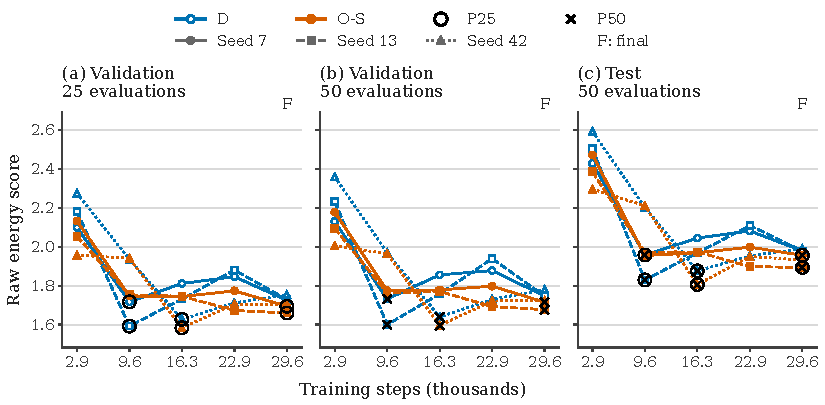
\includegraphics[width=\linewidth]{figures/checkpoints/fig_checkpoints.pdf}
 \caption{How the D/O-S comparison changes during training. The subplots show VAL with 25 DDIM evaluations, VAL with 50, and TEST with 50. Each point gives equal weight to months; ensembles contain 39 samples. Colors and open or filled markers distinguish D and O-S, while line styles and marker shapes distinguish seeds. Black rings mark the validation choice with 25 evaluations, P25; crosses mark the choice with 50, P50. Both choices coincide for all six fits. F marks the common final update. Validation and test scores concern different windows, and model choice precedes the additional TEST analysis.}
 \label{fig:checkpoints}
\end{figure}

\section{A stationary hidden Markov model with a known distribution}
\label{app:oracle}

\begin{figure}[t]
 \centering
 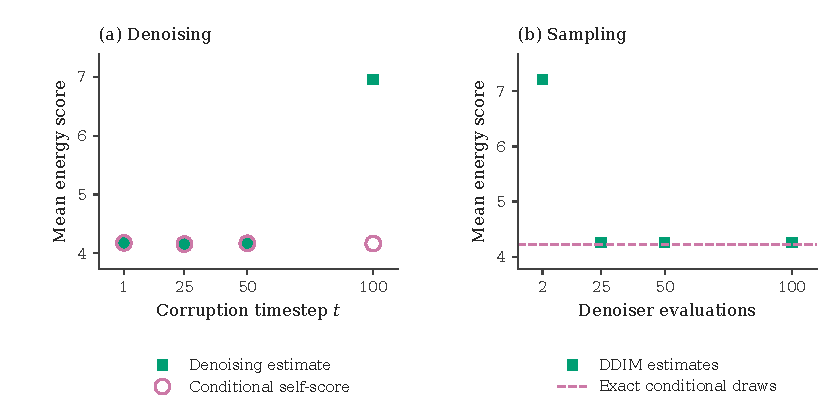
\includegraphics[width=\linewidth]{figures/hmm/fig_hmm.pdf}
\caption{The stationary hidden Markov model separates residual size from distributional accuracy. Subplots (a,b) use the same 36 cases at each timestep, each with 128 conditional paths and independent noise. (a) Squares give the mean energy score of denoising estimates; open circles estimate the expected score of the conditional distribution using an independent random stream. (b) Mean absolute residual on a logarithmic axis. The first two means are near floating point precision. The estimator uses one denoiser evaluation at $t=1$ and two at the other timesteps. (c) Complete DDIM sampling uses 39 samples on each of 288 windows, a separate evaluation population. The dashed line gives the score of independent samples from the exact conditional distribution. All scores are finite Monte Carlo estimates.}
 \label{fig:hmm}
\end{figure}

This example makes the conditional distribution available by calculation, so denoising and sampling can be examined without error from fitting a network. The two states, $z_0$ and $z_1$, are magnetic statistics that obey the same identity as the solar wind data. For $\alpha\in\{0,1,2\}$, define $c_j=j-3$ for $j=1,\ldots,5$ and $d_\alpha=\sqrt{1+2\alpha^2}$. The vectors that produce the two states are
\begin{equation}
 B_j^{(0)}=\frac{(1,\alpha c_j,0)}{d_\alpha},\qquad
 B_j^{(1)}=\frac{2(1+2\alpha c_j,\,2-2\alpha c_j,\,2+\alpha c_j)}{3d_\alpha}.
 \label{eq:toystates}
\end{equation}
The mean squared field magnitudes are $Q_0=1$ and $Q_1=4$ in HMM units for every $\alpha$. Thus, the geometry and magnitude variance can change while each state retains its own value of $Q$, preserving the difference between the states. Standardization gives equal weight to the six states and uses $B_{\mathrm{ref}}^2=2.5$; these values are set before evaluation.

A two-state Markov chain determines the sequence, with switching probability $p\in\{0.1,0.25,0.5\}$ and transition matrix $T_p=\bigl(\begin{smallmatrix}1-p&p\\p&1-p\end{smallmatrix}\bigr)$. Twelve hidden states connect the left state $a$ to the right state $b$, giving thirteen transitions. Stationarity sets $\Pr(a)=1/2$ and $\Pr(b\mid a,p)=(T_p^{13})_{ab}$. The hidden sequence is then sampled conditional on these two states.

Each record has 48 bins spanning four hours. The 18 bins before the missing hour repeat the left state's statistics, and the 18 bins after it repeat the right state's statistics. This context reveals $\alpha$ and the two end states, while the switching probability $p$ remains unknown. The twelve intervening bins follow a Markov trajectory conditional on the end states.

Inference averages over the three possible switching probabilities, each with prior probability $1/3$. The end states give weights proportional to $\Pr(p)(T_p^{13})_{ab}$. At each denoiser evaluation, the likelihood of the current noisy input further updates these weights. The calculation and the prediction methods have the same available information.

For posterior probability $q$ of state 1, define $\kappa_\alpha=[1+2\sqrt{1+\alpha^2}+2\sqrt{1+4\alpha^2}]/5$. The posterior mean has residual
\begin{equation}
 R_{\mathrm{obs}}\bigl((1-q)z_0+qz_1\bigr)
 =q(1-q)\frac{11/3-\kappa_\alpha^2}{1+2\alpha^2}.
 \label{eq:toymean}
\end{equation}
The coefficient is positive at $\alpha=0,1$ and negative at $\alpha=2$. Both states satisfy the identity, yet their posterior mean has a nonzero residual whenever $0<q<1$. A squared residual penalty assigns a positive loss to this exact posterior mean. The example gives a magnetic realization of the nonlinear expectation problem discussed by \citet{bastek2025pidm}.

Evaluation uses 32 paths for each switching probability. Reusing each path for the three values of $\alpha$ gives 288 windows with the same hidden state sequences across geometries. This arrangement permits comparison of sampling accuracy as the geometry changes.

Table~\ref{tab:oracle} compares sampling methods on these 288 windows, using stationary end states, the same available information and 39 samples per method. The approximate samplers start from the same noise. Independent samples from the exact conditional distribution provide the first row: this distribution minimizes the expected energy score, while the finite estimate in the table varies with Monte Carlo error. DDIM with two denoiser evaluations has a substantially higher score; the scores with 25, 50 and 100 evaluations lie close to the exact-distribution estimate. The earlier independent-endpoint design forms a separate sensitivity analysis.

\begin{table}[h]
\centering
\caption{Primary energy scores for 288 stationary hidden Markov windows. The exact conditional distribution averages over the unknown switching probability. DDIM uses the exact denoiser with the evaluation counts shown. All scores come from finite ensembles.}
\label{tab:oracle}
\begin{tabular}{lc}
\toprule
Procedure & Energy score \\
\midrule
Exact conditional draws & 4.2287 \\
Two evaluations of exact denoiser & 7.2183 \\
Exact denoiser, 25 evaluations & 4.2591 \\
Exact denoiser, 50 evaluations & 4.2586 \\
Exact denoiser, 100 evaluations & 4.2567 \\
\bottomrule
\end{tabular}
\end{table}

The denoising comparison asks two related questions. For a particular noisy input, it compares estimates with the posterior conditional on that input. For a given context of end states and vector geometry, it also examines estimates across new hidden paths and independent noise. Exact conditional samples use a separate random stream. Each calculation covers 36 cases at each of four timesteps, giving 144 cases in total. A posterior concentrated on one path at low noise can be the correct response to that input. This differs from assessing the distribution across repeated paths and noise in Figure~\ref{fig:hmm}(a).

\subsection{Training diffusion models on the same HMM}

The learned models test how these residual objectives behave during training. Each fit uses 4{,}096 windows generated at seed 106 by cycling through the nine $(\alpha,p)$ combinations, a U-Net with channel widths 32/64/64, batches of 128, and 5{,}000 optimizer updates at seed 7. The remaining optimizer and diffusion settings follow Appendix~\ref{app:protocol}. Table~\ref{tab:learnedtoy} compares nine fits to the stationary chain with 50 DDIM evaluations for sampling. M and S denote the mean estimate and the estimate from two denoiser evaluations defined in Appendix~\ref{app:protocol}. At both coefficients, the identity penalty gives primary scores close to D, whereas omitting the variances gives higher scores with either estimator. These comparisons concern one training seed and its existing samples; variation across training seeds remains outside this comparison. The earlier models with independent end states belong to a separate analysis.

\begin{table}[ht]
\centering
\caption{Nine diffusion fits to the stationary hidden Markov model after 5{,}000 optimizer updates at seed 7. Evaluation uses 288 windows and 39 samples per window; clipping retains the model state and samples. Raw $|R|$ is the mean absolute residual of the observation identity in HMM units. The inequality column gives the percentage of generated bins that fail a moment inequality beyond rounding tolerance, separately from the equality residual. Coverage averages the five primary coordinates and twelve positions. The independent exact conditional ensemble has 100\% coverage for the inclusive nominal 90\% intervals.}
\label{tab:learnedtoy}
\begin{tabular}{lrrrrrr}
\toprule
 & & \multicolumn{2}{c}{Energy score} & \multicolumn{3}{c}{Raw samples} \\
Procedure & $c_R$ & Raw & Clipped & $|R|$ & \parbox[c]{19mm}{\centering Bins failing inequalities (\%)} & 90\% coverage (\%) \\
\midrule
D & 0 & 4.2607 & 4.2609 & 0.0126 & 27.5 & 94.5 \\
I-M & 0.0005 & 4.3283 & 4.3285 & 0.2861 & 26.6 & 84.3 \\
I-M & 0.005 & 4.6021 & 4.6022 & 0.7050 & 26.6 & 81.2 \\
I-S & 0.0005 & 4.4991 & 4.4993 & 0.6262 & 26.0 & 77.5 \\
I-S & 0.005 & 4.8020 & 4.8020 & 1.0086 & 29.2 & 74.6 \\
O-M & 0.0005 & 4.2604 & 4.2605 & 0.0122 & 27.8 & 94.7 \\
O-M & 0.005 & 4.2544 & 4.2545 & 0.0095 & 27.4 & 95.3 \\
O-S & 0.0005 & 4.2593 & 4.2595 & 0.0120 & 27.8 & 94.8 \\
O-S & 0.005 & 4.2551 & 4.2553 & 0.0094 & 27.4 & 95.9 \\
\bottomrule
\end{tabular}
\end{table}

The two comparisons separate the estimate used in the training loss from the distribution produced at inference. Two evaluations of the exact denoiser can give a small residual and a poor energy score. The learned O-S model, sampled with 50 evaluations, has a score close to D in this experiment. Thus, the toy exposes a limitation of the residual estimate as evidence of distributional accuracy; its training consequence also depends on the data loss and the sampling procedure.

Discreteness also matters for interval coverage. The exact conditional ensembles in Table~\ref{tab:oracle} give coverage of 100.0\% and 97.49\% under the nominal 90\% and 50\% conventions, with mean widths 1.4581 and 1.3485 in standardized coordinates. The intervals include their endpoints, so tied values can raise coverage above the values expected for a continuous distribution. This explains why the nominal percentages alone would mischaracterize calibration in this toy.

\section{Prediction scores and interval coverage}
\label{app:details}

Here and in Appendix~\ref{app:strata}, Gaussian denotes interpolation with a Gaussian residual fit on TRAIN. Gaussian regression instead uses the wider available context; Table~\ref{tab:main} and Appendix~\ref{app:extension} present that model separately.

The primary energy score evaluates the joint prediction for the missing hour in 60 coordinates. Subtracting each quantity's TRAIN mean and dividing by its TRAIN scale makes field values in nT and scalar variance in nT$^2$ dimensionless. The score combines distance to the withheld record with separation between predictions, as defined in the main text. The true conditional distribution minimizes its population expectation \citep{gneiting2007strictly}. The term ``energy score'' denotes this statistical criterion; magnetic energy density is a separate physical quantity assessed below.

Each seed in Table~\ref{tab:seeds} corresponds to one training run. All runs reach the common final update, while validation chooses the checkpoint used for prediction. It makes this choice separately for raw predictions and predictions after clipping. Coverage is calculated from each model's own ensemble before averaging across seeds.

The intervals in Table~\ref{tab:contrasts} quantify how score differences vary across the test years for the existing fits and samples. Each comparison uses the same resampled years for both methods. With seed 7003, 10{,}000 resamples take either the twenty individual years or the ten consecutive groups of two years, from 2005--2006 through 2023--2024. Repeated occurrences of a year each contribute their months, preserving equal weight per month.

For O-S minus D, the relative intervals are $[-0.016766,0.014049]$ for individual years and $[-0.016842,0.012995]$ for groups of two years. Both fit inside the original range of two percent in either direction. The intervals for O-S versus I-S and I-S versus D span both improvement and deterioration. These are marginal intervals for the existing fits and samples, based on twenty years or ten groups. Their interpretation across solar cycles depends on temporal stability, and their nominal coverage over repeated studies remains unverified. Variation from new training runs is outside this resampling calculation.

\begin{table}[ht]
\centering
\caption{Validation choice, primary energy score and raw nominal 90\% coverage for each training seed. Raw predictions and predictions after clipping choose their checkpoints separately. Scores use standardized coordinates. Coverage is calculated from each ensemble of 39 samples, then averaged over five primary quantities and twelve hidden positions.}
\label{tab:seeds}
\begin{tabular}{llrrrrr}
\toprule
 & & \multicolumn{2}{c}{Chosen updates} & \multicolumn{2}{c}{Energy score} & Raw coverage \\
Method & Seed & Raw & Clipped & Raw & Clipped & (\%) \\
\midrule
D & 7 & 9560 & 29636 & 1.9575 & 1.9147 & 67.2 \\
D & 13 & 9560 & 9560 & 1.8297 & 1.8213 & 75.9 \\
D & 42 & 16252 & 16252 & 1.8758 & 1.8724 & 75.4 \\
I-S & 7 & 9560 & 9560 & 1.9423 & 1.9385 & 63.3 \\
I-S & 13 & 22944 & 22944 & 1.8954 & 1.8826 & 66.5 \\
I-S & 42 & 16252 & 16252 & 1.8070 & 1.8071 & 78.2 \\
O-S & 7 & 29636 & 29636 & 1.9558 & 1.9116 & 60.4 \\
O-S & 13 & 29636 & 29636 & 1.8934 & 1.8824 & 70.5 \\
O-S & 42 & 16252 & 16252 & 1.8056 & 1.8045 & 79.2 \\
G5 & 7 & 29636 & 29636 & 1.7236 & 1.7239 & 75.9 \\
G5 & 13 & 29636 & 29636 & 1.7853 & 1.7889 & 67.1 \\
G5 & 42 & 16252 & 16252 & 1.8453 & 1.8404 & 84.0 \\
\bottomrule
\end{tabular}
\end{table}

\begin{table}[ht]
\centering
\caption{Primary energy score differences, first method minus second. Unsuperscripted procedures use raw predictions; $c$ denotes clipping with a separate validation choice of checkpoint. The first four rows assess the original O-S superiority criterion; the others are secondary comparisons. Year and Two-year give marginal percentile 95\% intervals using the same resampled years for both methods, with individual years or consecutive groups of two years. Seed differences appear in the order 7, 13, 42. Gaussian denotes interpolation with a Gaussian residual.}
\label{tab:contrasts}
\setlength{\tabcolsep}{1.8pt}
\begin{tabular}{@{}lrrrr@{}}
\toprule
Contrast & Mean & Year & Two-year & Seed differences \\
\midrule
O-S $-$ D & -0.0028 & $[-0.0346,0.0242]$ & $[-0.0345,0.0233]$ & $(-0.0018,0.0637,-0.0702)$ \\
O-S $-$ D$^c$ & 0.0154 & $[-0.0024,0.0312]$ & $[-0.0034,0.0320]$ & $(0.0410,0.0721,-0.0669)$ \\
O-S $-$ G5 & 0.1002 & $[0.0712,0.1391]$ & $[0.0671,0.1422]$ & $(0.2322,0.1080,-0.0398)$ \\
O-S $-$ G5$^c$ & 0.1005 & $[0.0716,0.1396]$ & $[0.0677,0.1420]$ & $(0.2319,0.1045,-0.0348)$ \\
O-S $-$ I-S & 0.0033 & $[-0.0236,0.0349]$ & $[-0.0259,0.0431]$ & $(0.0135,-0.0020,-0.0015)$ \\
I-S $-$ D & -0.0061 & $[-0.0562,0.0330]$ & $[-0.0720,0.0410]$ & $(-0.0152,0.0656,-0.0688)$ \\
O-S $-$ Gaussian & -0.2402 & $[-0.5298,-0.0481]$ & $[-0.4539,-0.0882]$ & $(-0.1694,-0.2318,-0.3196)$ \\
\bottomrule
\end{tabular}
\end{table}

\subsection{Interval coverage, width, and score contributions}

Interval coverage reveals a difference between O-S and D despite their similar primary scores. In Table~\ref{tab:calibration}, O-S falls farther below nominal 90\% coverage by 2.8 percentage points, exceeding the prespecified threshold of two percentage points. Gaussian interpolation is closer to nominal at 90\% but substantially overcovers at 50\%. These averages describe overall coverage; calibration for particular available measurements remains to be assessed.

The differences also vary across quantities. O-S covers scalar variance more often than D, but covers each vector component and mean magnitude less often, as Table~\ref{tab:channelcoverage} shows. The energy score assesses their joint distribution across all 60 coordinates. Coordinate coverage instead locates errors in the individual quantities and positions.

G5's mean score improvement over D is largely accounted for by its larger spread term. Its mean distance to the withheld measurements is also slightly smaller. Figure~\ref{fig:calibration}(a) separates these contributions using the checkpoints that minimize raw validation score, the same 60 standardized coordinates, and equal month and seed weights.

The contribution of each term differs by seed. At seed 13, G5 reduces both distance to the measurements and spread, with the larger decrease in distance lowering the score. At seed 42, both terms increase, and the larger increase in spread lowers the score. These are arithmetic explanations of the existing predictions. G5 changes both the generated representation and the training loss, so their separate effects on learning remain unresolved.

\paragraph{Where observations fall outside the intervals.}
G5's nominal 90\% intervals cover only 40.5\% of the $v_s$ observations. To show the direction of the errors, the calculation separates observations below the second smallest of 39 samples, between the second and 38th inclusive, and above the 38th. When ensemble members and the observation are independent samples from the same continuous conditional distribution, each observation rank is equally likely. The expected fractions are then 5\%, 90\% and 5\%.

For each fit, all TEST windows contribute: fractions are averaged over positions, then over windows in each month, with equal weights for months and for fits of the same method. Examining each variable and each tail complements the proper score \citep{gneiting2007calibration}: an overall coverage percentage can combine errors in opposite directions.

Across the three fits, 49.0\% of observations fall below G5's $v_s$ intervals and 10.5\% above them. Figure~\ref{fig:calibration} shows why the mean alone is incomplete: errors are predominantly below the intervals at seeds 7 and 13, but above them at seed 42. D has the same reversal at seed 42. For O-S, the mean fractions are 37.7\% below and 8.4\% above.

For G5's $v_s$ intervals, the fraction below exceeds the fraction above by 38.4 percentage points. The 95\% interval is $[36.2,40.6]$, using 10{,}000 resamples of years and the same years for both fractions. Repeated occurrences of each year retain their weight. The difference uses percentages before rounding. This contrast quantifies temporal variation for the existing models, checkpoint choices and samples; new fits or new checkpoint choices would add other sources of uncertainty.

Gaussian regression covers 98.1\% of $v_s$ observations, with 0.6\% below and 1.2\% above its intervals. Those wide intervals accompany a worse primary energy score. Reading coverage, width and score together distinguishes how often intervals contain the data, how concentrated the predictions are, and their performance under a proper scoring rule. Both temporal resampling schemes cover every method and coordinate.

\begin{figure}[ht]
 \centering
 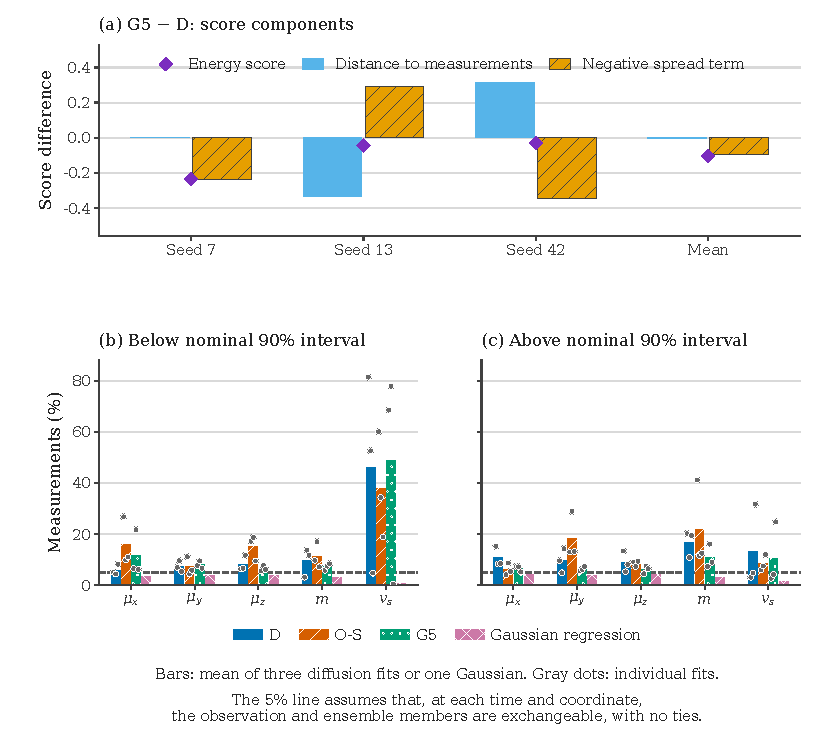
\includegraphics[width=\linewidth]{figures/calibration/fig_calibration.pdf}
\caption{Why scores and interval coverage differ. Diffusion results use the checkpoints that minimize raw validation score. (a) G5 minus D for each seed and their mean. The change in distance to the withheld record, less the change in the spread term, gives the energy score difference. Both terms use 60 coordinates standardized on TRAIN; spread is half the mean distance between distinct predictions. (b,c) Fractions of observations below and above nominal 90\% intervals for the five primary quantities. Bars average three diffusion fits or show one Gaussian ensemble. Gray dots show seeds 7, 13 and 42 from left to right. The dashed 5\% line assumes that, at each time and coordinate, the observation and ensemble members are exchangeable, with no ties. Months receive equal weight. This analysis uses the existing TEST ensembles after the original results were available.}
 \label{fig:calibration}
\end{figure}

\begin{table}[ht]
\centering
\caption{Marginal continuous ranked probability scores, interval coverage and width for the five primary quantities. Scores and widths use dimensionless standardized values; coverage is in percent. Results average hidden positions, months and three diffusion seeds. Each other method uses one ensemble. Clipped rows apply the clipping map. Diffusion procedures choose checkpoints separately before and after clipping, except the D row that retains the weights from the raw procedure. Gaussian denotes interpolation with a Gaussian residual.}
\label{tab:calibration}
\setlength{\tabcolsep}{4pt}
\begin{tabular}{lrrrrr}
\toprule
 & & \multicolumn{2}{c}{50\% intervals} & \multicolumn{2}{c}{90\% intervals} \\
Procedure & \parbox[c]{27mm}{\centering Continuous ranked probability score} & Coverage (\%) & Width & Coverage (\%) & Width \\
\midrule
D raw & 0.1753 & 35.5 & 0.2878 & 72.8 & 0.8709 \\
D clipped & 0.1721 & 33.5 & 0.2814 & 71.0 & 0.8617 \\
D clipped, raw weights & 0.1734 & 36.1 & 0.2883 & 73.5 & 0.8722 \\
I-S raw & 0.1745 & 32.7 & 0.2785 & 69.4 & 0.8315 \\
I-S clipped & 0.1735 & 32.8 & 0.2789 & 69.6 & 0.8319 \\
O-S raw & 0.1729 & 31.9 & 0.2691 & 70.0 & 0.8213 \\
O-S clipped & 0.1701 & 32.6 & 0.2685 & 71.1 & 0.8195 \\
G5 raw & 0.1634 & 38.1 & 0.3137 & 75.7 & 0.9308 \\
G5 clipped & 0.1624 & 38.4 & 0.3128 & 75.8 & 0.9287 \\
Gaussian raw & 0.1960 & 76.4 & 0.6262 & 94.3 & 1.5822 \\
Gaussian clipped & 0.1935 & 68.6 & 0.5512 & 93.6 & 1.3933 \\
Interpolation raw & 0.1993 & 0.0 & 0.0000 & 0.0 & 0.0000 \\
Interpolation clipped & 0.1993 & 0.0 & 0.0000 & 0.0 & 0.0000 \\
Persistence raw & 0.2697 & 0.1 & 0.0000 & 0.1 & 0.0000 \\
Persistence clipped & 0.2697 & 0.1 & 0.0000 & 0.1 & 0.0000 \\
\bottomrule
\end{tabular}
\end{table}

\begin{table}[ht]
\centering
\caption{Nominal 90\% coverage in percent for each primary quantity before clipping. Hidden positions, months and diffusion seeds receive equal weight in their respective averages. Gaussian denotes interpolation with a Gaussian residual.}
\label{tab:channelcoverage}
\begin{tabular}{lrrrrr}
\toprule
Procedure & $\mu_x$ & $\mu_y$ & $\mu_z$ & $m$ & $v_s$ \\
\midrule
D & 83.6 & 83.2 & 83.0 & 73.8 & 40.6 \\
I-S & 82.2 & 74.8 & 80.7 & 74.3 & 34.9 \\
O-S & 78.2 & 74.6 & 76.4 & 67.0 & 53.9 \\
G5 & 82.1 & 85.9 & 87.6 & 82.2 & 40.5 \\
Gaussian & 93.1 & 93.5 & 92.2 & 94.1 & 98.5 \\
Interpolation & 0.0 & 0.0 & 0.0 & 0.0 & 0.0 \\
Persistence & 0.1 & 0.2 & 0.1 & 0.0 & 0.0 \\
\bottomrule
\end{tabular}
\end{table}

\begin{samepage}
Changing the coordinates in the score changes the question it asks. The vector score in Table~\ref{tab:alternative} uses 36 standardized coordinates; adding $m$, $v_s$ and $v_v$ gives 72. Although $v_v$ follows from the other quantities for realizable statistics, including it changes distances and the relative influence of errors. The resulting scores have different scales and can rank methods differently. Gaussian interpolation has a lower mean vector score than D, I-S and O-S. G5 has the lowest mean primary score over five quantities, while its rank changes when $v_v$ enters the score.

The magnetic energy calculation assesses a different aspect of the prediction. For realizable statistics, $m^2+v_s$ equals the mean squared magnitude of the five vector averages, each over one minute. Conversion to T$^2$ and division by $2\mu_0$ give the magnetic energy density represented by those averages; variation within the original minute averages is absent. The same scalar transformation is applied to every predicted bin and averaged over the missing hour for each ensemble member. CRPS compares this scalar ensemble with the energy density of the withheld record. Interpreting each predicted value as the energy density of vectors with the other predicted moments depends on their joint realizability. CRPS and interval width have units of J\,m$^{-3}$, shown as multiples of $10^{-12}$ in Table~\ref{tab:alternative}. Raw Gaussian interpolation has the lowest CRPS for this quantity among the procedures in that table. Clipping brings the moments into the ranges in Equation~\ref{eq:support} to rounding tolerance, but its effect on the score depends on how the predictive distribution changes.
\end{samepage}

\begin{table}[ht]
\centering
\caption{Scores for alternative magnetic quantities. The vector and six-coordinate energy scores use 36 and 72 standardized coordinates. The last three columns assess the mean magnetic energy density over the missing hour, computed for each ensemble member from $m^2+v_s$. This quantity retains the energy represented by vector averages over one minute and excludes variation within those averages. Raw rows evaluate the same scalar even when the other predicted moments are inconsistent. Continuous ranked probability score and interval width are in $10^{-12}$ J\,m$^{-3}$; coverage is in percent. Validation chooses model states separately for raw and clipped diffusion predictions. Gaussian denotes Gaussian interpolation.}
\label{tab:alternative}
\setlength{\tabcolsep}{4pt}
\begin{tabular}{@{}lrrrrr@{}}
\toprule
 & \multicolumn{2}{c}{Energy score} & \multicolumn{3}{c}{Resolved magnetic energy density} \\
Procedure & Vector & \parbox[c]{17mm}{\centering Six coordinates} & \parbox[c]{27mm}{\centering Continuous ranked probability score} & 90\% coverage (\%) & 90\% width \\
\midrule
D raw & 1.6351 & 2.1528 & 2.8599 & 74.3 & 6.2166 \\
D clipped & 1.6222 & 2.5726 & 2.7568 & 68.5 & 6.6024 \\
I-S raw & 1.6435 & 2.1590 & 2.4664 & 72.4 & 6.6657 \\
I-S clipped & 1.6435 & 2.8791 & 2.3049 & 73.1 & 6.8576 \\
O-S raw & 1.6316 & 2.1503 & 2.9225 & 65.3 & 6.5977 \\
O-S clipped & 1.6316 & 2.3863 & 2.7461 & 72.2 & 6.6863 \\
G5 raw & 1.5740 & 2.4959 & 1.8961 & 82.2 & 6.8060 \\
G5 clipped & 1.5740 & 2.4285 & 1.9066 & 82.4 & 6.8757 \\
Gaussian raw & 1.5909 & 2.7342 & 1.0816 & 93.8 & 6.1012 \\
Gaussian clipped & 1.5909 & 4.2146 & 2.5465 & 64.8 & 11.2941 \\
Interpolation raw & 1.9834 & 2.8920 & 1.2771 & 0.0 & 0.0000 \\
Interpolation clipped & 1.9834 & 4.6381 & 1.2771 & 0.0 & 0.0000 \\
Persistence raw & 2.7925 & 3.6601 & 2.6284 & 0.0 & 0.0000 \\
Persistence clipped & 2.7925 & 3.6601 & 2.6284 & 0.0 & 0.0000 \\
\bottomrule
\end{tabular}
\end{table}

\subsection{Vector increments at the edges and inside the missing interval}

At the two edges of the missing hour, vector increments connect indices 17 to 18 and 29 to 30. Table~\ref{tab:geometry} gives their mean magnitudes and the RMSE of individual predictions, calculated across 39 samples within each window and then averaged over months and seeds. This RMSE combines error of the predictive mean with predictive spread. It describes edge behavior, while the proper scores assess distributional accuracy.

The withheld record has mean increment magnitudes of 1.0460 nT at the left edge, 1.0539 nT at the right edge, and 1.0831 nT inside the missing hour. Interpolation imposes a smooth connection between the available measurements. Comparison with the withheld increments tests how well that smooth connection represents the actual variation.

The variogram score examines dependence through differences between coordinates, using exponent $1/2$ \citep{scheuerer2015variogram}. This calculation weights 175 pairs equally: 55 connect adjacent times within a primary quantity and 120 connect different quantities at the same time. For pair $(i,j)$, let $d_k=|x_{k,i}-x_{k,j}|^{1/2}$. The contribution is $(|y_i-y_j|^{1/2}-\bar d)^2-s_d^2/K$, with $K=39$ and variance $s_d^2$ computed using divisor $K-1$. The squared term compares the transformed difference in the measurements with the ensemble mean. For independent samples, that estimate has variance $\operatorname{Var}(d_k)/K$; subtracting $s_d^2/K$ removes its upward Monte Carlo bias in expectation. The final score averages these contributions. It complements the energy score by emphasizing differences between coordinates.



\begin{table}[ht]
\centering
\caption{Vector increments and variogram scores before clipping. Mean increment magnitudes and RMSE across predictions in each window use nT. The variogram uses the 175 standardized coordinate pairs defined in the text and the finite-ensemble bias correction. Clipping retains the vector increments when the model weights stay the same, while its changes to $m$ and $v_s$ can alter the variogram. D also changes vector predictions through the separate validation choice of checkpoint at seed 7. Gaussian denotes interpolation with a Gaussian residual.}
\label{tab:geometry}
\begin{tabular}{lrrrrrr}
\toprule
 & & \multicolumn{3}{c}{Mean increment magnitude} & \multicolumn{2}{c}{Root mean square error} \\
Procedure & Variogram & Left edge & Right edge & Internal & Left edge & Right edge \\
\midrule
D & 0.0524 & 1.3121 & 1.3581 & 0.8560 & 1.8164 & 1.8323 \\
I-S & 0.0521 & 1.3309 & 1.4224 & 0.8156 & 1.8059 & 1.8854 \\
O-S & 0.0524 & 1.3111 & 1.3296 & 0.7635 & 1.7974 & 1.7990 \\
G5 & 0.0490 & 1.3717 & 1.3830 & 1.0789 & 1.8893 & 1.8958 \\
Gaussian & 0.0905 & 1.5737 & 1.5587 & 1.5718 & 2.1020 & 2.1114 \\
Interpolation & 0.0658 & 0.2518 & 0.2518 & 0.2518 & 1.0373 & 1.0309 \\
Persistence & 0.1003 & 0.0000 & 3.2730 & 0.0000 & 1.0460 & 3.1140 \\
\bottomrule
\end{tabular}
\end{table}

\subsection{Numerical precision when transforming observations}
\label{app:numerics}

Table~\ref{tab:roundtrip} measures arithmetic error in the 5{,}760 hidden observation bins, without evaluating a model. The affine transform is fitted on TRAIN and applied in float64. One route retains float64 values; the other stores them in float32 before the scoring decoder performs the inverse transform in float64. The route using five coordinates then derives $v_v$. All routes satisfy the inequalities for these observations, even without a rounding allowance. Exact algebraic completion can make the computed equality residual zero while leaving rounding error in the primary coordinates.

\begin{table}[t]
\centering
\caption{Numerical error after normalization and its inverse. Maximum $|\Delta u|$ is the largest absolute change among the five standardized primary coordinates in all hidden bins. Equality residuals are in nT$^2$. Deriving $v_v$ makes the computed residual zero without removing rounding error from the primary coordinates.}
\label{tab:roundtrip}
\begin{tabular}{lrrr}
\toprule
Representation & \parbox[c]{16mm}{\centering Maximum $|\Delta u|$} & Mean $|R_{\rm obs}|$ & \parbox[c]{16mm}{\centering Maximum $|R_{\rm obs}|$} \\
\midrule
Original float64 & 0 & $8.476\times10^{-15}$ & $3.326\times10^{-13}$ \\
Float64 normalization and inverse & $1.271\times10^{-15}$ & $8.987\times10^{-15}$ & $5.573\times10^{-13}$ \\
Float32, six coordinates & $4.977\times10^{-7}$ & $1.571\times10^{-6}$ & $6.268\times10^{-5}$ \\
Float32, derived $v_v$ & $4.977\times10^{-7}$ & 0 & 0 \\
\bottomrule
\end{tabular}
\end{table}

\section{Variation across spacecraft, years, and magnetic conditions}
\label{app:strata}

Table~\ref{tab:strata} examines how the primary score varies with spacecraft, calendar period and magnetic conditions. For each subgroup, the score averages first over windows within a month and then equally over the months present. Combining subgroup scores by window count can give a different result from the overall test score.

Spacecraft and calendar period vary together in this sample. In 2020--2024, 119 windows use Wind and only one uses ACE, so the spacecraft comparison also includes temporal variation. The calendar groups themselves span different phases of the solar cycle. The intervals from resampling years describe the existing predictions and remain exploratory, without adjustment for the number of comparisons.

Two further comparisons group windows by conditions during the missing hour. The 480 TEST windows are divided into thirds by mean withheld magnitude, using thresholds of 3.9350 and 5.7891 nT, or by mean internal vector increment, using thresholds of 0.6134 and 1.2055 nT. Each division gives 160 windows per group; none of the values equals a threshold.

Grouping by the withheld outcome changes the distribution represented by each subset. Even a forecast that correctly describes outcomes conditional on the available measurements can rank differently under a proper score after this additional selection. The opposite signs of O-S minus D at low and high magnitude describe the particular TEST cases in those groups. Interpreting them as a prediction benefit conditional on field strength depends on an evaluation that accounts for the outcome selection. Each row of Table~\ref{tab:years} covers one year. Intervals from resampling years apply to groups spanning multiple years.

\begin{table}[ht]
\centering
\caption{Raw primary energy score across spacecraft, calendar periods, and thirds of TEST defined by withheld mean magnitude or mean internal vector increment. The last column gives a marginal 95\% interval for O-S minus D from resampling years. Scores use standardized primary coordinates and average the same three diffusion fits. The groups defined by withheld values describe outcomes after selection; a claim about conditional predictive superiority depends on accounting for that selection. ACE denotes the Advanced Composition Explorer.}
\label{tab:strata}
\setlength{\tabcolsep}{5pt}
\begin{tabular}{@{}lrrrrrr@{}}
\toprule
Stratum & Windows & D & O-S & G5 & O-S $-$ D & Year interval \\
\midrule
Wind (52) & 335 & 1.7136 & 1.7119 & 1.6159 & -0.0017 & $[-0.0382,0.0303]$ \\
ACE (71) & 145 & 1.8597 & 1.9008 & 1.7886 & 0.0411 & $[-0.0009,0.0869]$ \\
2005--2009 & 120 & 1.9817 & 2.0219 & 1.9051 & 0.0403 & $[0.0158,0.0638]$ \\
2010--2015 & 144 & 1.7735 & 1.7728 & 1.6890 & -0.0007 & $[-0.0416,0.0415]$ \\
2016--2019 & 96 & 1.6349 & 1.6220 & 1.5657 & -0.0129 & $[-0.0543,0.0237]$ \\
2020--2024 & 120 & 2.1330 & 2.0928 & 1.9545 & -0.0403 & $[-0.1384,0.0293]$ \\
Magnitude, lower third & 160 & 1.1777 & 1.2324 & 1.1010 & 0.0547 & $[0.0195,0.0835]$ \\
Magnitude, middle third & 160 & 1.4606 & 1.4747 & 1.4339 & 0.0140 & $[-0.0044,0.0310]$ \\
Magnitude, upper third & 160 & 3.3910 & 3.3366 & 3.1849 & -0.0544 & $[-0.1089,-0.0023]$ \\
Increment, lower third & 160 & 0.8924 & 0.9174 & 0.8255 & 0.0250 & $[-0.0056,0.0560]$ \\
Increment, middle third & 160 & 1.4411 & 1.4416 & 1.3768 & 0.0005 & $[-0.0392,0.0434]$ \\
Increment, upper third & 160 & 3.2522 & 3.2284 & 3.0924 & -0.0238 & $[-0.0804,0.0271]$ \\
\bottomrule
\end{tabular}
\end{table}

\begin{table}[ht]
\centering
\caption{Annual raw primary energy scores in standardized coordinates. Each row uses 24 test windows, averages the year's two TEST months and then the three diffusion seeds. Gaussian denotes the shared ensemble from Gaussian interpolation. These results describe the existing fits and cases. A single annual row provides no variation across years for a resampling interval.}
\label{tab:years}
\begin{tabular}{lrrrrr}
\toprule
Year & D & I-S & O-S & G5 & Gaussian \\
\midrule
2005 & 3.3402 & 3.4233 & 3.3349 & 3.1962 & 3.3435 \\
2006 & 1.8130 & 1.8449 & 1.8911 & 1.8222 & 2.0005 \\
2007 & 1.5185 & 1.6045 & 1.5749 & 1.4551 & 2.1359 \\
2008 & 1.8584 & 1.8789 & 1.8882 & 1.7878 & 2.1347 \\
2009 & 1.3782 & 1.4624 & 1.4206 & 1.2640 & 1.5893 \\
2010 & 1.2774 & 1.3131 & 1.2785 & 1.2081 & 1.5417 \\
2011 & 2.5543 & 2.5698 & 2.5144 & 2.3807 & 2.2021 \\
2012 & 1.3628 & 1.3747 & 1.4155 & 1.3091 & 1.6150 \\
2013 & 1.1809 & 1.2399 & 1.2585 & 1.1578 & 1.4643 \\
2014 & 2.5162 & 2.4384 & 2.4978 & 2.4404 & 2.4855 \\
2015 & 1.7493 & 1.7088 & 1.6719 & 1.6383 & 1.7181 \\
2016 & 1.9325 & 1.8200 & 1.8618 & 1.7919 & 1.9331 \\
2017 & 1.7522 & 1.7971 & 1.7414 & 1.7083 & 2.0006 \\
2018 & 1.5171 & 1.5611 & 1.5522 & 1.4413 & 1.6696 \\
2019 & 1.3378 & 1.3602 & 1.3326 & 1.3214 & 1.6536 \\
2020 & 1.5016 & 1.5137 & 1.5409 & 1.4375 & 1.6264 \\
2021 & 1.3806 & 1.4460 & 1.4136 & 1.3686 & 1.5898 \\
2022 & 1.9837 & 2.0144 & 1.9358 & 1.9206 & 1.9962 \\
2023 & 2.5198 & 2.3208 & 2.5221 & 2.1314 & 2.1605 \\
2024 & 3.2793 & 2.9392 & 3.0514 & 2.9142 & 5.6425 \\
\bottomrule
\end{tabular}
\end{table}

\subsection{Directional cancellation with thresholds from TRAIN}

Directional cancellation occurs when the norm of the mean vector is smaller than the mean of the individual magnitudes. The cancellation analysis examines whether the variance identity penalty behaves differently under these conditions. For each bin, define $C=(m^2-\|\mu\|^2)/m^2$, with $C=0$ when $m=0$, and $A=(m^2-\|\mu\|^2)/B_{\mathrm{ref}}^2$. Both measures are dimensionless: $C$ expresses cancellation relative to the bin's squared mean magnitude, while $A$ uses the common TRAIN scale.

The groups use mean $C$ over the 36 available bins or mean $A$ over the twelve hidden bins. High cancellation means strictly above the TRAIN 75th percentile: 0.044395 for the available intervals and 0.022696 for the missing interval. Every one of the 122{,}309 overlapping training windows contributes equally to these thresholds, whereas normalization uses distinct bins. The rules predate the implementation, which followed inspection of the primary results; the analysis is exploratory.

Window means of $Q/B_{\mathrm{ref}}^2$ define the energy groups. Here $Q=m^2+v_s$ is the magnetic second moment in nT$^2$, and the ratio is dimensionless; this physical quantity is distinct from the statistical energy score. TRAIN quartile thresholds are $(0.349809,0.571606,1.078729)$ for the available intervals and $(0.343518,0.563106,1.069013)$ for the missing interval. A value equal to an energy threshold enters the higher energy group. A value equal to the cancellation threshold enters the rest group.

The 21 groups comprise the full test set, high cancellation and the rest, and combinations of cancellation with energy conditions. All 18 procedures are evaluated in each group. Scores give equal weight to the months present and then average the three diffusion seeds.

\begin{samepage}
High cancellation in the available measurements identifies 128 windows across all twenty years. O-S minus D is $-0.0256$, with a 95\% interval of $[-0.0740,0.0147]$ from resampling years. All three seed differences are negative, while the interval includes zero. O-S minus G5 is $0.0573$, with interval $[0.0053,0.1246]$, and O-S minus D is $0.0114$ in the remaining 352 windows. G5 has a lower mean score in this group, while the O-S versus D interval spans zero. The group uses information available to the model; cancellation can still vary with other magnetic conditions.
\par
\end{samepage}

High cancellation during the missing hour identifies 121 windows. O-S minus D is $-0.0128$, with interval $[-0.0858,0.0629]$, compared with $0.0068$ in the remaining 359 windows. Although the thresholds come from TRAIN, assignment to these TEST groups uses the withheld values. The score comparison is consequently conditional on outcome selection.

Combining high cancellation during the missing hour with the lowest energy quartile leaves seven windows from five years. Their scores describe this small subset of TEST outcomes. Interpreting them as evidence of conditional predictive superiority depends on accounting for the rule that uses withheld values to form the groups.

\section{Clipping samples to satisfy moment constraints and Gaussian regression}
\label{app:extension}

\subsection{Algebraic completion and clipping of existing samples}

Applying algebraic completion and clipping to existing ensembles separates their effects from changes introduced by training. Both operations use the same models, samples and windows, with model weights chosen by raw validation score. Algebraic completion derives $v_v$ from the other five coordinates, preserving those values and their primary energy score. Training G5 changes both the generated representation and the loss, so its comparison combines those changes with algebraic completion.

Clipping acts on the primary coordinates themselves. It retains $\mu$, raises $m$ to $r=\|\mu\|$ when necessary, and then clips $v_s$ to $[0,1.5m^2+2.5r^2]$ using the new value of $m$. Deriving $v_v$ completes a realizable set of moments. A second application preserves them to the stated arithmetic tolerance. The construction specifies a feasible adjustment, without a claim of minimum displacement.

The change in score is limited by how far clipping moves the samples. For primary samples $X=(x_1,\ldots,x_K)$ and observation $y$,
\begin{equation}
 \left|\operatorname{ES}(CX,y)-\operatorname{ES}(X,y)\right|
 \le \frac{2}{K}\sum_{i=1}^K\|Cx_i-x_i\|.
 \label{eq:movement}
\end{equation}
By the reverse triangle inequality, each score term changes in absolute value by at most the mean sample displacement. Adding these contributions gives Equation~\ref{eq:movement}; the argument applies to convex and nonconvex realizable sets. The bound concerns magnitude, so the score can increase or decrease. Distances use all 60 primary coordinates after TRAIN standardization and are dimensionless. Table~\ref{tab:operators} adds the change in distance to withheld measurements and subtracts the change in the spread term.

\begin{table}[ht]
\centering
\caption{Effects of clipping the same ensembles before any further model selection. Model weights, samples and windows are identical in each comparison; diffusion uses the models chosen by raw validation score. Months receive equal weight, followed by an average over three diffusion seeds or the one comparison ensemble. Distances use 60 primary coordinates standardized on TRAIN. Displacement is the mean distance moved by an ensemble member. The two term changes, with signs as shown, sum to the change in energy score before rounding.}
\label{tab:operators}
\begin{tabular}{lrrrr}
\toprule
Procedure & Displacement & $\Delta$ distance & $-\Delta$ spread term & $\Delta$ energy score \\
\midrule
D & 0.1254 & -0.00350 & -0.00287 & -0.00637 \\
I-S & 0.0997 & -0.00427 & -0.00119 & -0.00547 \\
O-S & 0.1521 & -0.01952 & 0.00080 & -0.01873 \\
G5 & 0.1055 & 0.00003 & -0.00038 & -0.00035 \\
Gaussian interpolation & 2.1403 & -0.32056 & 0.42478 & 0.10422 \\
\bottomrule
\end{tabular}
\end{table}

\begin{samepage}
The size of an inequality error distinguishes frequent small departures from large ones. Before allowing for rounding, a deficit is zero when the inequality holds and measures the departure when it fails; failure frequency counts such failures without regard to size. For G5, the 90th percentile of $\max(r-m,0)/B_{\mathrm{ref}}$ is calculated within each window and averages to 0.01648, compared with 0.34407 for Gaussian interpolation. For $\max(-v_s,0)/B_{\mathrm{ref}}^2$, the corresponding values are 0.000342 and 0.017372. Both deficits are dimensionless.

For each window, the percentile is calculated across its samples and hidden bins. These window percentiles are averaged within each month, then across months and seeds. Taking one percentile across all windows would be a different calculation. G5 and Gaussian interpolation both frequently fail the inequalities, yet clipping moves their samples by very different distances. G5's small score change coexists with many samples outside the realizable set.

\end{samepage}

\begin{samepage}
For D, Table~\ref{tab:operators} attributes an energy score change of $-0.00637$ to clipping the ensemble chosen by raw validation score. Choosing the model independently on VAL after clipping adds a further change of $-0.01183$; seed~7 is the only run for which the chosen training step changes. The raw and clipped scores in Table~\ref{tab:main} combine these two effects: altering the samples and choosing the model.

\end{samepage}

\begin{figure}[t]
 \centering
 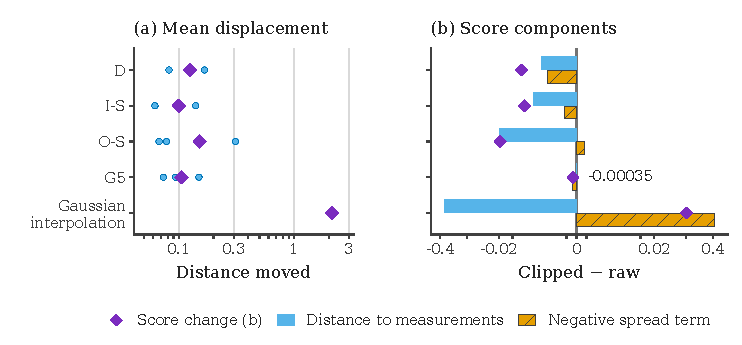
\includegraphics[width=0.90\linewidth]{figures/operator/fig_operator.pdf}
\caption{Clipping samples from models chosen by raw validation score. (a) Mean displacement in 60 standardized coordinates on a logarithmic axis. Blue circles show individual fits; purple diamonds show their mean or one Gaussian ensemble. (b) Solid bars show the change in distance to withheld values; striped bars show the change in the negative spread term. Their sum, the energy score change, appears as purple diamonds. The symmetric logarithmic axis is linear inside $\pm0.005$. Clipping changes D's score by $-0.0064$; choosing another checkpoint adds $-0.0118$.}
 \label{fig:operator}
\end{figure}

\subsection{Multivariate Gaussian regression}

Gaussian regression uses the measurements before and after the missing hour to estimate departures from interpolation. Its input $X$ contains all 216 standardized available coordinates; $Y$ contains the 60 primary residuals from interpolation between bins 17 and 30, divided by the corresponding TRAIN scales. Fitting $W$ and an unpenalized intercept $b$ on TRAIN minimizes $\|Y-XW-b\|_F^2/N+\lambda\|W\|_F^2$, with equal weight for all 122{,}309 overlapping windows.

The nine parameter combinations use $\lambda\in\{0.001,0.1,1\}$ and covariance $(1-\rho)S+\rho\operatorname{diag}(S)+10^{-6}I$, where $\rho\in\{0,0.5,1\}$ and $S$ is the empirical residual covariance with divisor $N$. Within each fit, the conditional mean varies with context and the residual covariance is common to all contexts. The first five coordinates have a Gaussian distribution; deriving $v_v$ gives a non-Gaussian distribution over all six. Positive definiteness makes the Gaussian covariance valid, while realizability remains a separate condition on its samples.

Common random innovations allow the nine parameter combinations to be compared using the same noise. Each VAL window uses 39 innovations from PCG64, identified by split, window, sample and seed 13. Validation minimizes energy score with equal month weights, separately before and after clipping; exact ties follow lexicographic $(\lambda,\rho)$ order. Both procedures choose $\lambda=0.1$ and $\rho=0$, with raw and clipped VAL scores of 1.73275 and 1.83453, respectively. These choices precede generation of the single TEST ensemble.

Compared with Gaussian interpolation, regression uses more available measurements, a different conditional mean fit and a different finite noise realization. Its score difference compares procedures that differ in all three respects.

G5 has a lower mean energy score than Gaussian regression: the difference is $-0.1503$, with a year interval of $[-0.2302,-0.0829]$ and an interval of $[-0.2105,-0.0913]$ from resampling groups of two years. Both intervals lie below zero. The corresponding O-S difference is $-0.0502$, with intervals $[-0.1336,0.0327]$ and $[-0.0913,-0.0080]$, respectively. For O-S, the interval spans zero when resampling individual years and excludes it when resampling groups of two years. Changing the temporal grouping changes the resampling distribution and the uncertainty in this comparison.

These marginal 95\% intervals measure temporal variation conditional on the three existing diffusion fits and one Gaussian ensemble. They use the original 10{,}000 temporal resamples, with the same years in both methods of each contrast. Variation from new fits, resampling seeds or repeating validation selection is outside these intervals. This later comparison uses a TEST period that had already been examined.

Before clipping, Gaussian regression has a vector energy score of 1.5728 over 36 standardized coordinates and a CRPS of $1.0497\times10^{-12}$ J\,m$^{-3}$ for mean resolved magnetic energy density. These scores concern different predictions and use different scales. Clipping leaves the vector predictions intact but raises the energy-density CRPS to $2.1873\times10^{-12}$ J\,m$^{-3}$. The mean displacement over all 60 standardized primary coordinates is 1.7733.

Clipping both Gaussian baselines reduces the spread term more than the mean distance to the withheld measurements. Subtracting the smaller spread term raises the primary energy score despite satisfaction of the moment constraints. Coverage near nominal describes how often marginal intervals contain measurements, and realizability describes which magnetic moments a sample can take. Each property describes one aspect of the predictions; accuracy of the full predictive distribution extends beyond either check.

\section{Penalty strength after training}
\label{app:fixedfinal}

The coefficient comparison evaluates every model after 29{,}636 training steps, using $c_R\in\{0,0.00005,0.0005,0.005\}$ at seeds 7, 13 and 42 in Table~\ref{tab:fixedfinal}. Zero gives D, and positive coefficients apply O-S's variance identity penalty. The final D and O-S models contribute six fits in total; the two additional coefficients contribute six more. Evaluation uses the same 480 windows, 39 samples and 50 DDIM evaluations as the main experiment. Each comparison before and after clipping uses the same model weights and random samples.

The training step for this comparison was specified in advance, and all twelve fits are included. Their TEST scores serve to compare the coefficients, without choosing a coefficient or an earlier model state from those scores. The comparison is exploratory: equal update counts can involve different amounts of computation, and differences in score may reflect convergence or overfitting.

\begin{table}[ht]
\centering
 \caption{Penalty coefficients compared after 29{,}636 training steps. Each row describes one fit and gives equal weight to the months present. Energy scores use the five primary quantities at twelve times in standardized coordinates. For samples before clipping, the remaining columns give mean absolute $R_{\mathrm{obs}}$ in nT$^2$, the percentage of bins failing a moment inequality beyond rounding tolerance, nominal 90\% coverage and mean interval width in standardized units. The inequality percentage excludes the equality test. All twelve fits are shown, with checkpoint and coefficient choices made independently of these scores.}
\label{tab:fixedfinal}
\begin{tabular}{lrrrrrr}
\toprule
 & \multicolumn{2}{c}{Energy score} & \multicolumn{4}{c}{Raw samples} \\
Coefficient / seed & Raw & Clipped & $|R|$ & \parbox[c]{19mm}{\centering Bins failing inequalities (\%)} & Coverage (\%) & Width \\
\midrule
0 / 7 & 1.9787 & 1.9147 & 3.5152 & 78.4 & 57.5 & 0.8018 \\
0 / 13 & 1.9778 & 1.9515 & 3.1092 & 68.1 & 67.9 & 0.8369 \\
0 / 42 & 1.9900 & 1.9847 & 4.2064 & 11.4 & 60.6 & 0.7955 \\
0.00005 / 7 & 2.0412 & 1.9714 & 3.5544 & 80.4 & 57.4 & 0.7830 \\
0.00005 / 13 & 1.8735 & 1.8653 & 2.8988 & 59.7 & 69.4 & 0.8347 \\
0.00005 / 42 & 1.9757 & 1.9702 & 3.8648 & 15.5 & 62.9 & 0.8396 \\
0.0005 / 7 & 1.9558 & 1.9116 & 2.8245 & 88.8 & 60.4 & 0.7797 \\
0.0005 / 13 & 1.8934 & 1.8824 & 2.3812 & 32.5 & 70.5 & 0.8112 \\
0.0005 / 42 & 1.9312 & 1.9284 & 3.1843 & 15.6 & 66.8 & 0.8634 \\
0.005 / 7 & 2.0224 & 1.9934 & 1.5068 & 69.1 & 57.2 & 0.7742 \\
0.005 / 13 & 2.0201 & 2.0114 & 1.7024 & 54.4 & 61.4 & 0.8303 \\
0.005 / 42 & 1.8119 & 1.8036 & 1.1243 & 44.2 & 68.6 & 0.7964 \\
\bottomrule
\end{tabular}
\end{table}

\begin{samepage}
Increasing the penalty lowers the mean absolute residual in Figure~\ref{fig:fixedfinal}, but the mean energy score first falls and then rises. The strongest penalty gives the smallest residual; the original coefficient gives the lowest mean score. At $c_R=0.005$, the score is lower than D's at seed 42 and higher at seeds 7 and 13. Across seeds, a smaller residual can accompany either a better or a worse predictive score.
\par
\end{samepage}

\begin{figure}[t]
 \centering
 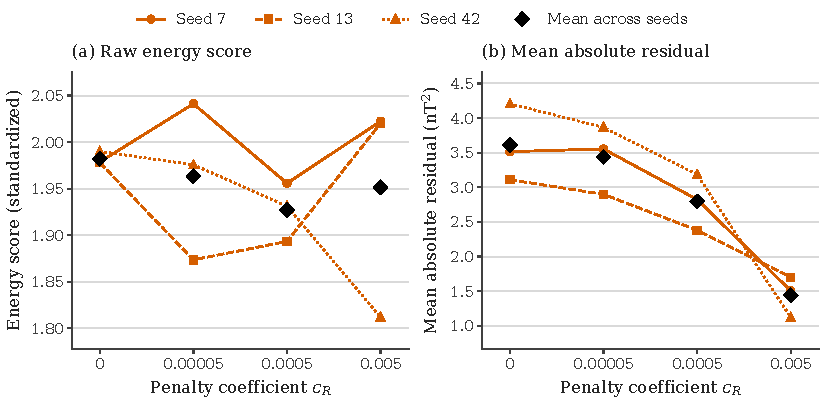
\includegraphics[width=\linewidth]{figures/fixed_final/fig_fixed_final.pdf}
 \caption{Energy score and residual of the variance identity after 29{,}636 training steps for the twelve models in Table~\ref{tab:fixedfinal}. Lines connect each seed's four coefficient settings; solid black diamonds show the mean across three seeds. The horizontal axis treats the coefficient settings as equally spaced categories. The left subplot gives raw energy score in standardized primary coordinates, and the right gives mean absolute $R_{\mathrm{obs}}$ in nT$^2$. Each model value gives equal weight to the months present.}
 \label{fig:fixedfinal}
\end{figure}

\begin{samepage}
At the original coefficient, O-S has a lower energy score than D at the end of all three training runs. Choosing each model by raw validation score gives a different comparison, with O-S minus D changing sign across seeds. These exploratory results show that the D/O-S comparison depends on the stage of training evaluated; its persistence across additional fits is untested.
\par
\end{samepage}

\section{Related work on physical constraints in prediction and generation}

Solar wind reconstruction can address different quantities. Gaussian process regression estimates upstream plasma and magnetic conditions at Mars between MAVEN observations, with uncertainty that depends on the available sampling \citep{azari2024virtual}. For incomplete magnetic records, feedforward networks estimate second-order structure functions directly, describing variation across time separations \citep{wrench2022statistics}. Diffusion has also been used to generate future coronal EUV images conditional on earlier images \citep{francisco2024corona}. Here, prediction concerns the joint distribution of magnetic moments throughout a missing hour, conditional on measurements before and after it. The moments retain fluctuation amplitudes in each bin while leaving the ordering of its minute vectors unspecified.

\citet[Section 3.3 and Appendix A.6.1]{bastek2025pidm} distinguish a residual at the denoiser mean from a residual at a sample, and demonstrate collapse when training uses the residual alone. Using an exact denoiser in the HMM makes it possible to examine the approximation from two denoiser evaluations without error from learning the denoiser. The solar wind experiments address the related question through comparisons across training stages and through algebraic completion or clipping of the same samples. The predictive score measures the distributional effect of those operations separately from their effect on the residual.

Algebraic completion also appears in physical emulators that produce one prediction for each input. \citet{beucler2021constraints} compare training on all outputs, including those from conservation layers, with training only on direct outputs and completing the rest algebraically. G5 applies the latter construction to a conditional generator, with changes to both its generated representation and training loss. Deriving $v_v$ after sampling preserves the primary score because that score uses the other five quantities. In climate downscaling, exact aggregation and nonnegativity impose distinct constraints, and predictive accuracy requires separate assessment \citep{harder2023hard}.

Nonlinear aggregation also enters physical observation models. In land surface temperature downscaling, PGDM compares arithmetic averaging with the fourth root of the mean fourth power of temperature \citep{zhang2025pgdm}. The latter rule neglects variation in emissivity. PGDM conditions on geophysical variables, trains with MSE, and measures error in physical consistency during evaluation.

WIND uses diffusion forcing for pretraining and moment matching for posterior guidance to reconstruct weather trajectories from observations that include spatial and temporal averages \citep{aich2026wind}. For guidance, the clean state conditional on the noisy state is approximated by a Gaussian. Its covariance is then propagated through a local linearization of the observation operator. PGDM and WIND place aggregation in the observation model, with training and inference that differ from the residual penalty examined here.

The weight given to a residual can also adapt during training. PILD models residuals with a Laplace likelihood whose scale depends on their magnitude. For conditional tasks, it aligns representations with the output of an encoder whose weights remain fixed during diffusion training \citep{zeng2026pild}. The scale calculation approximates conditional moments of residual magnitude from minibatch statistics with exponential averaging. Inference uses two denoiser evaluations, compared with 50 here.

Physics-Based Flow Matching integrates the flow to $t=1$ before evaluating residuals and combines gradients of the flow matching and residual losses through ConFIG \citep{baldan2025physics}. The present experiment keeps $c_R$ constant throughout training; adaptive objectives and gradient combinations fall outside its scope.

\section{Two examples of magnetic reconstruction}
\label{app:imputation}

Figures~\ref{fig:imputation120} and \ref{fig:imputation360} illustrate two missing hours from TEST in physical units. Windows 120 and 360, counting from zero, are the midpoints of the two halves of the ordered list of 480 windows. Position determines their choice independently of model error, although TEST had already been examined. Diffusion uses seed 7, the first declared seed. Minimizing the raw validation score gives training step 9560 for D and 29636 for O-S and G5; Gaussian regression uses the fit chosen by validation and the noise realization from seed 13. These examples illustrate individual reconstructions, with uncertain representativeness across TEST.

Every method receives the same surrounding measurements and is compared with the same withheld values. The colored curve joins the marginal medians of 39 samples at each time and coordinate. After sorting those samples in increasing order, values 2 and 38 form the inclusive nominal 90\% interval. The joined medians can be irregular and can differ from every sampled trajectory. These curves and intervals concern each time and quantity separately; simultaneous coverage of an entire trajectory is a separate property. Thin lines show the first three sampled trajectories, ensemble members 0, 1 and 2.

The horizontal axes mark the starts of bins of five minutes, relative to the missing hour. Figures~\ref{fig:imputation120} and \ref{fig:imputation360} show predictions before clipping. Within each figure, the methods share a vertical scale for each quantity. For $v_s$, a symmetric logarithmic scale accommodates both small measured variances and Gaussian predictions outside the physical range. The reconstructed statistics describe five minutes of measurements; different sequences of minute averages can produce the same statistics.

Available measurements retain their values during sampling. The plots show them separately from the twelve predicted bins, with short line breaks from $-5$ to $0$ minutes and from $55$ to $60$ minutes. Each neighboring bin contains a different set of five vectors. The variance identity constrains the moments inside a bin, while the conditional model learns their dependence across time. The elevated variance predictions are model errors; Figure~\ref{fig:imputationdetail} shows them on linear scales.

The scalar variance $v_s$ is the variance of the magnitudes of five vector averages, each taken over one minute. In both examples, diffusion generally places its median above the withheld variance, which often falls outside the nominal intervals. In TEST window 120, every diffusion method covers $v_s$ in zero of the twelve hidden bins. In window 360, D, O-S and G5 cover zero, one and two bins, respectively. The aggregate coverage results show the same shortfall from nominal coverage for this quantity.

Gaussian regression's much wider intervals contain all twelve withheld values in both windows. Its residual covariance is common to every context, and its distribution places probability on negative $v_s$, which is physically impossible. The frequency of these particular error patterns across TEST, and their origin during training, remain uncertain.

\begin{figure}[p]
 \centering
 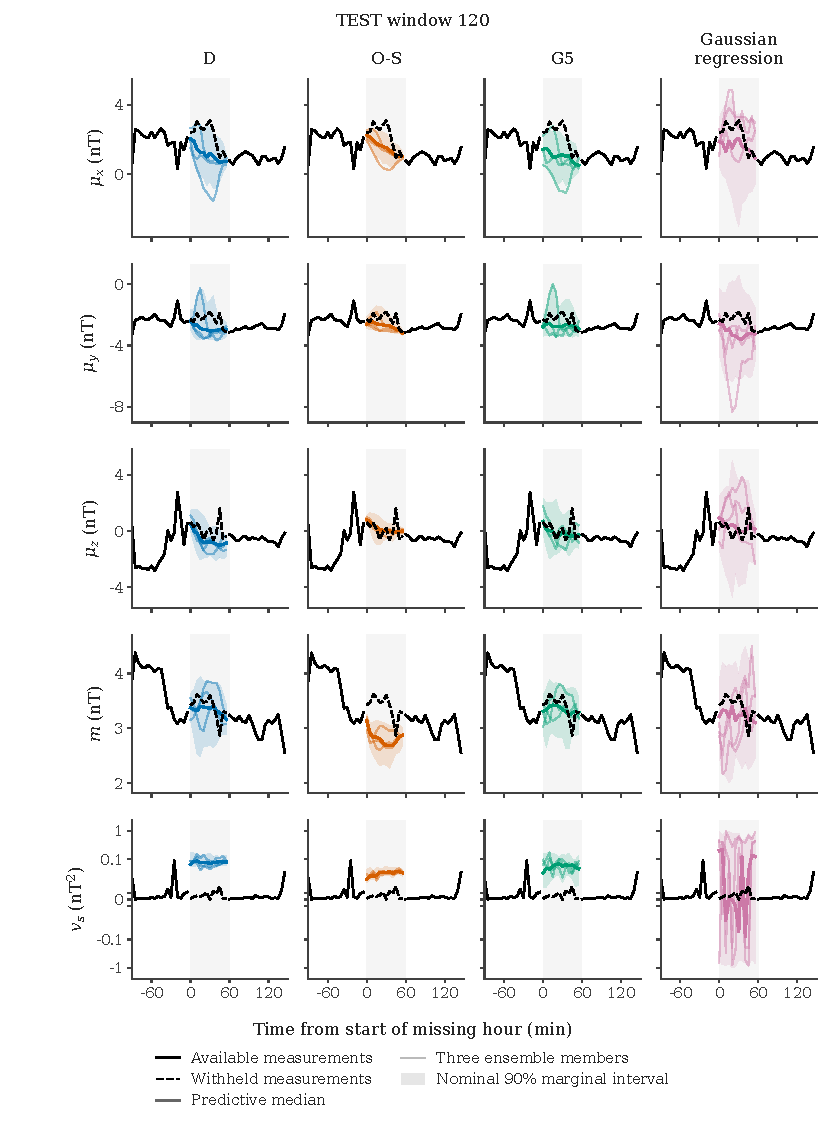
\includegraphics[width=0.95\linewidth]{figures/imputation/case_120/fig_imputation.pdf}
 \caption{Reconstruction from ACE measurements on 3 August 2010, TEST window 120. The missing hour runs from 13:30 to 14:30 UTC on the OMNI arrival-time grid. Columns compare D, O-S, G5 and Gaussian regression, with model weights chosen by validation; rows show the five primary magnetic statistics in physical units. All samples appear before clipping. Diffusion uses seed 7 and Gaussian regression uses seed 13. Solid black lines show 90 minutes of available observations on each side of the shaded missing hour, and dashed black lines show the withheld measurements. Colored lines show marginal medians, bands show nominal 90\% intervals, and thin lines show ensemble members 0, 1 and 2. Times mark the starts of bins of five minutes relative to the missing hour. The $v_s$ axis is linear within $0.05$ nT$^2$ of zero and logarithmic outside, so equal vertical distances can represent different absolute errors in that row. Negative variance predictions are visible. Appendix~\ref{app:imputation} explains the case choice and the construction of the intervals.}
 \label{fig:imputation120}
\end{figure}

\begin{figure}[p]
 \centering
 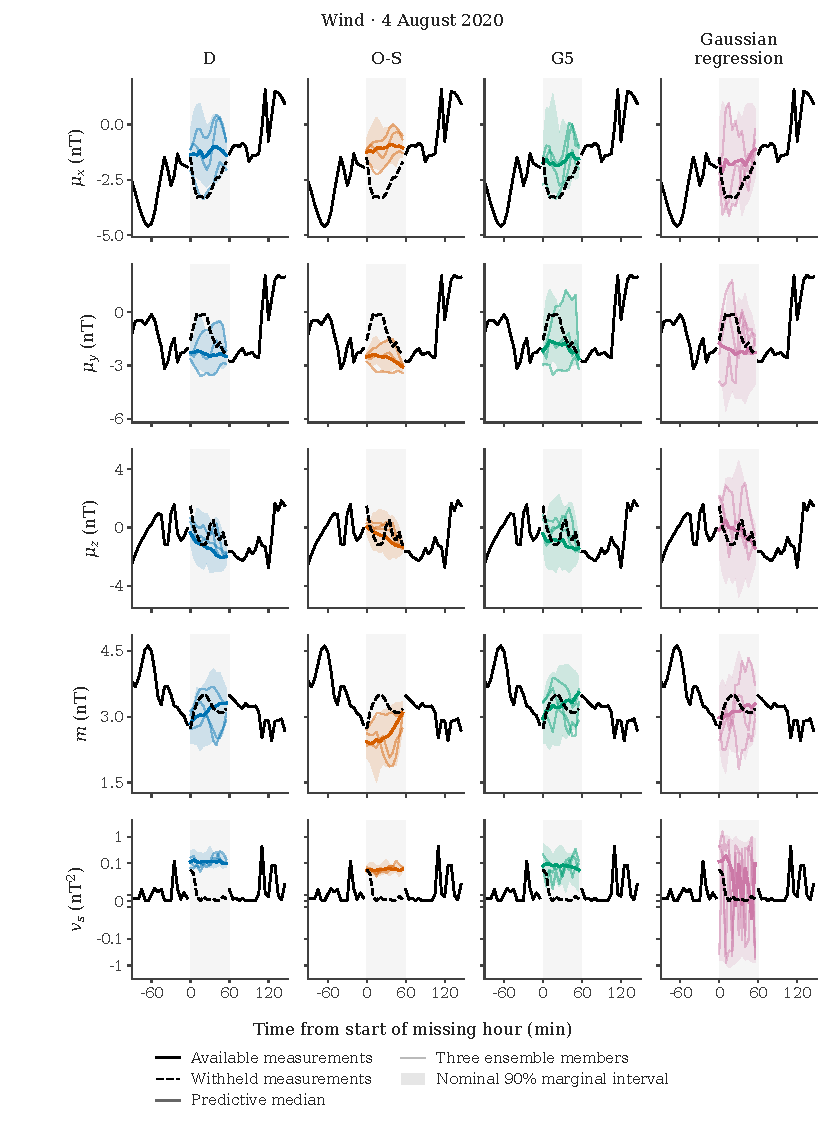
\includegraphics[width=0.95\linewidth]{figures/imputation/case_360/fig_imputation.pdf}
 \caption{Reconstruction from Wind measurements on 4 August 2020, TEST window 360. The missing hour runs from 18:30 to 19:30 UTC on the OMNI arrival-time grid. Methods, seed choices, units and line styles follow Figure~\ref{fig:imputation120}. Each method's own ensemble determines its predictive intervals.}
 \label{fig:imputation360}
\end{figure}

\begin{figure}[p]
 \centering
 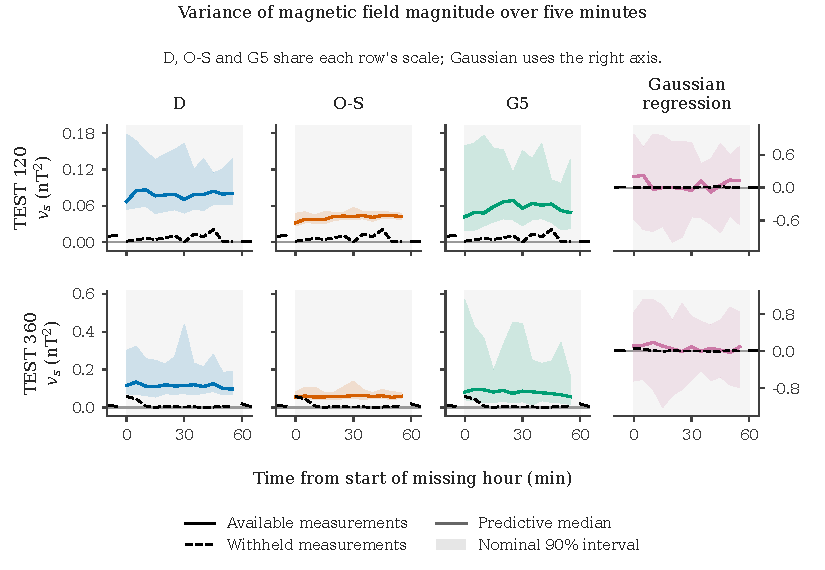
\includegraphics[width=\linewidth]{figures/imputation/detail/fig_imputation.pdf}
 \caption{Variance of magnetic field magnitude in bins of five minutes during the same two missing hours. D, O-S and G5 share a linear scale in each row; Gaussian regression uses a separate linear scale on the right. Band heights and vertical distances are comparable on a common scale. Every subplot includes all measurements, medians and interval ends in its axis limits. Solid black lines show available observations, and dashed black lines show withheld measurements. Colored lines show empirical medians, and bands show nominal 90\% marginal predictive intervals from all 39 samples. Times mark bin starts relative to the missing hour. The horizontal gray line marks zero; predictions below it are physically impossible because variance is nonnegative. Gaussian regression has much wider intervals that contain the observations.}
 \label{fig:imputationdetail}
\end{figure}


\end{document}
